\documentclass[a4paper]{report}

\usepackage{fullpage} % Package to use full page
\usepackage{parskip} % Package to tweak paragraph skipping
\usepackage{tikz} % Package for drawing
\usepackage{amsmath}
\usepackage{float}
% \usepackage{hyperref}
\usepackage{pdfpages} % For inserting entire pages from a PDF
\usepackage{graphicx} % For including images

\title{Zero to Hero: WiMo}
\author{Niels Savvides}
\date{\today}

\begin{document}

\maketitle

\chapter{Analyse in 1 veranderlijke: enkele aspecten}

\subsection{Continuiteitseigenschappen van functies}

Functie $f(x)$ is contine over $]a,b[$ als:
\begin{enumerate}
	\item $f(x)$ bestaat in elk punt
	\item de limiet van $f(x)$ bestaat in elk punt
\end{enumerate}

\textbf{Continue afgeleide}: $f(x)$ is continue (zie hierboven) en $f'(x)$ bestaat in elk punt.
Dit kan:
\begin{enumerate}
	\item gladde functies zijn: elk afgeleide is continue
	\item stuksgewijs: $f(x)$ heeft een singulariteit, maar het bestaat in deel intervallen $]a, c[$ $]c, b[$
\end{enumerate}

\begin{figure}[!htbp]
	\begin{center}
		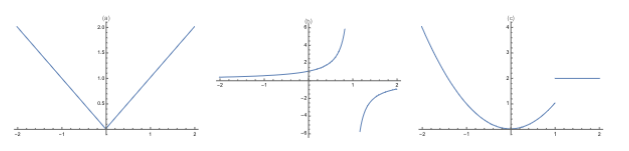
\includegraphics[width=8cm]{./images/continu.png}
	\end{center}
	\caption{a) Continue functie, stukgewijs continue afgeleide (als je afleid krijg je een singulareit) b) Heeft een singulaireit, dus stukgewijs continue, stukgewijs glad continue afleidbaar c) Deze is glad stukgewijs continue afleidbaar, is ook stukgewijs continue }
\end{figure}


\subsection{Taylorontwikkeling}
\label{sec:taylor}

We willen zaken gaan benaderen. Hiervoor gebruiken we:

$ f(x) = f(a) + f'(a)(x-a) + \frac{f''(a)}{2!}(x-a)^2 + \frac{f'''(a)}{3!}(x-a)^3 + ... $

waarbij $a$ het \textbf{werkpunt} is.

Veel voorkomende Taylorontwikkelingen:

See Figure \ref{fig:veel_voorkomend_taylor}.

\begin{figure}[htbp!]
	\centering
	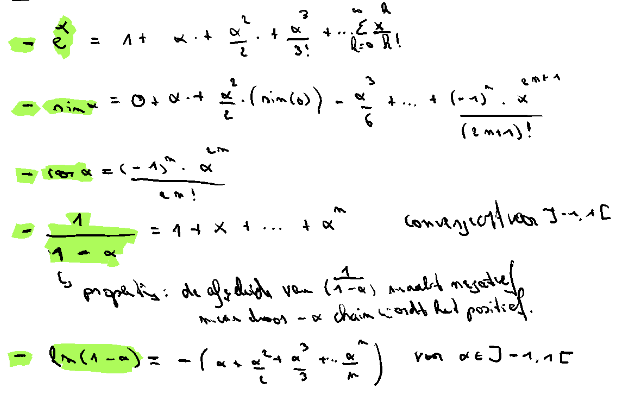
\includegraphics[width=0.8\textwidth]{assets/veel_voorkomend_taylor.png}
	\caption{Simply use the formulas}
	\label{fig:veel_voorkomend_taylor}
\end{figure}

\subsection*{Storingsrekening}

Zie Figuur \ref{fig:storing_solution}.

Of Maple solution \ref{sol:storing}.

\begin{figure}[!htbp]
	\centering
	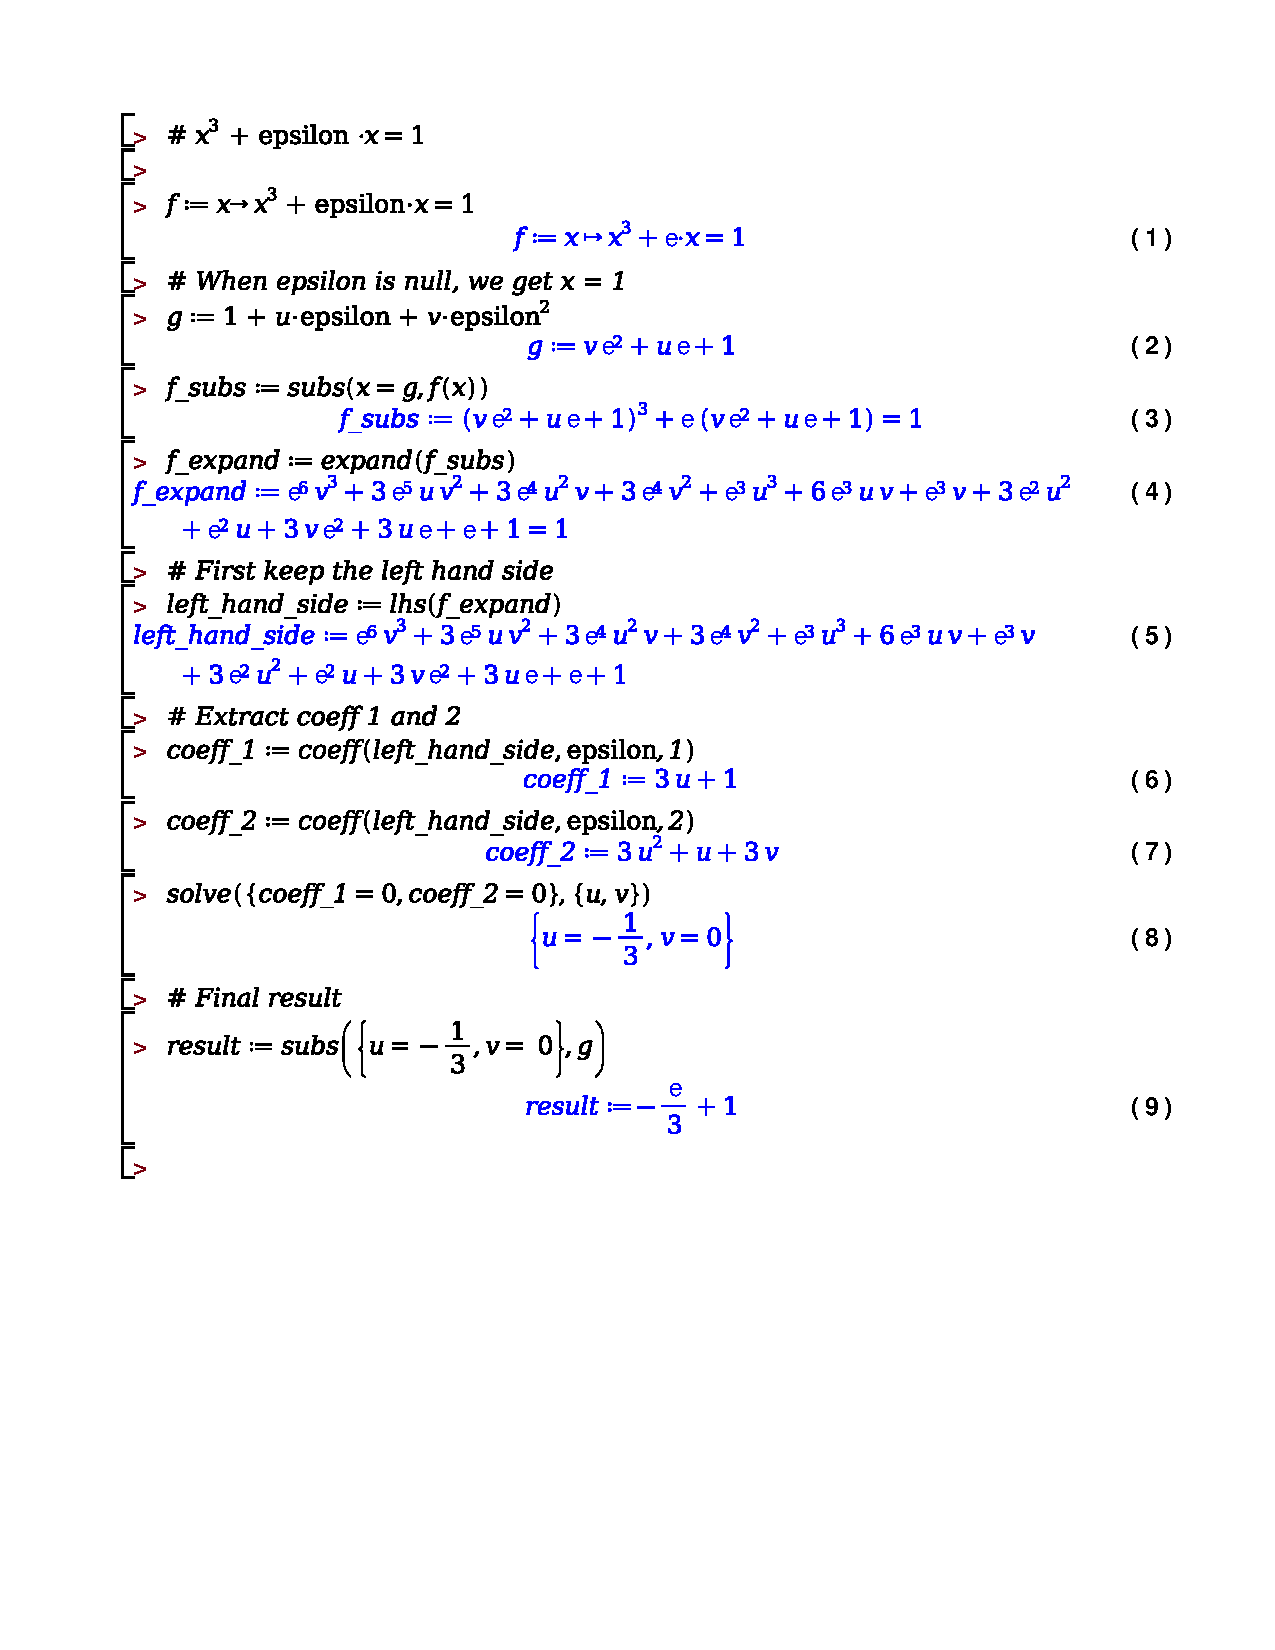
\includegraphics[width=\textwidth]{./storing.pdf}
	\caption{Maple solution}
	\label{sol:storing}
\end{figure}

\begin{figure}[htbp!]
	\centering
	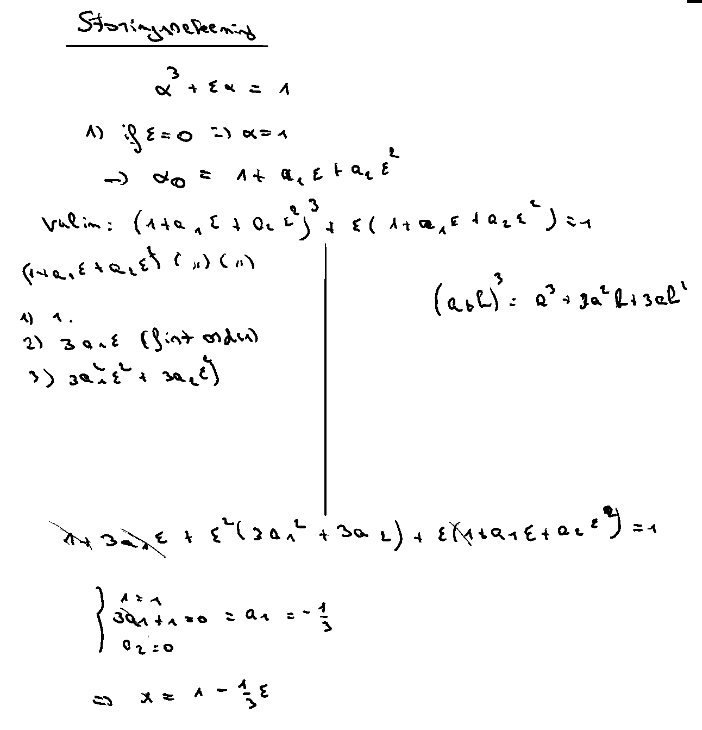
\includegraphics[width=0.8\textwidth]{assets/storing_solution.png}
	\caption{1. Merk op dat als epsilon 0 is, dan is x = 1. Dus we benaderen value 1: $1 + \epsilon . u + \epsilon^2 . v$. Vul dit in the main equation. Gebruik maple om dit op te lossen en vul $u$ en $v$ in $x_1$}
	\label{fig:storing_solution}
\end{figure}

\subsection{Twee eenvoudige differentiaalvergelijkingen}

\subsubsection{Eerste orde differentiaalvergelijking}

$y'(x) = \lambda y(x)$

Als we dit uitwerken krijgen we:

$ln(y(x)) = \lambda x + C$

$y(x) = e^{\lambda x + C} = e^C e^{\lambda x} = C e^{\lambda x}$ met $C = y(0)$

$y(x) = y(0) e^{\lambda x}$

\subsubsection*{Radioactief verval}

Zie Figuur \ref{fig:radio_solution}.

\begin{figure}[htbp!]
	\centering
	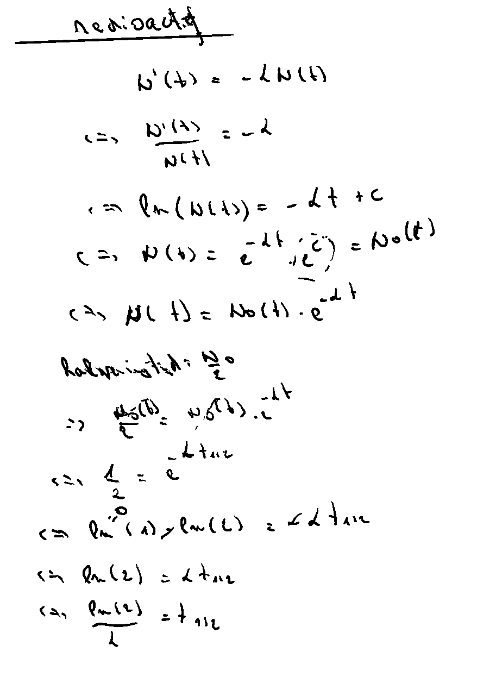
\includegraphics[width=0.8\textwidth]{assets/radio_solution.png}
	\caption{Vindt eerst de differentiaalvergelijking (zie eerste differentiaalvergelijking). Dan kunnen we de oplossing gelijkstellen aan $N_0 / 2$. Werk dit uit en je hebt $t_{1/2}$ gevonden}
	\label{fig:radio_solution}
\end{figure}

\subsubsection{Tweede orde differentiaalvergelijking}

$y''(x) = \lambda y(x)$

Hierbij heb je 3 gevallen:

1. $\lambda > 0$: $y(t) = A e^{\sqrt{\lambda} t} + B e^{-\sqrt{\lambda} t}$

2. $\lambda = 0$: $y(t) = A + Bt$

3. $\lambda < 0$: $y(t) = A cos(\sqrt{-\lambda} t) + B sin(\sqrt{-\lambda} t)$

\subsubsection{Complexe getallen}

Algemene vorm: $z = a + bi$

waarbij $a$ reeel, $b$ imaginair en $i^2 = -1$

\textbf{inverse}: $(a + bi)^{-1} = \frac{a - bi}{a^2 + b^2}$

\textbf{complement}: $z = a + bi \rightarrow z^* = a - bi$

\textbf{modulus}: $|z| = \sqrt{a^2 + b^2}$

in \textbf{polaire vorm}:

$e^{i\theta} = cos(\theta) + i sin(\theta)$ (Dit kan via Taylor bewezen worden (zie oefeningen))

Okey, nu nog een paar goniometrische formules:

$sin^2(x) + cos^2(x) = 1$

$sin(x) = \frac{e^{ix} - e^{-ix}}{2i}$

$sin(2x) = 2sin(x)cos(x)$

$cos(x) = \frac{e^{ix} + e^{-ix}}{2}$

$cos(2x) = cos^2(x) - sin^2(x)$

\subsubsection{Hoofdstelling van de algebra}

Als we een kwadratisch veelterm hebben: $ax^2 + bx + c = 0$

Dan vinden we de nulpunten (oplossingen) met:

$x_1 = \frac{-b + \sqrt{b^2 - 4ac}}{2a}$

$x_2 = \frac{-b - \sqrt{b^2 - 4ac}}{2a}$

met $b = -4*a*c$ vinden we de discriminant.

\chapter{Lineare Algebra}

\subsection{Lineare onafhanlijkheid}

\textbf{Lineare onafhankelijkheid} betekent dat de vectoren niet op een lijn liggen. Dit betekent dat de determinant van de matrix niet 0 is.
Maar ook dat de vectoren niet een lineaire combinatie van elkaar zijn.

\begin{figure}[htbp!]
	\centering
	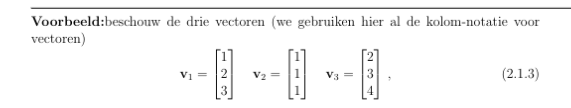
\includegraphics[width=0.8\textwidth]{images/ex_lin_on.png}
	\caption{1. Merk op dat als epsilon 0 is, dan is x = 1. Dus we benaderen value 1: $1 + \epsilon . u + \epsilon^2 . v$. Vul dit in the main equation. Gebruik maple om dit op te lossen en vul $u$ en $v$ in $x_1$}
\end{figure}

$v_1, v_2, v_3$ zijn lineair onafhankelijk. Maar $v_1$ en $v_2$ bijvoorbeeld, vormen een lineaire combinatie van $v_3$

\subsection{Inproduct, Norm, Orthogonaliteit}

- \textbf{Inproduct}: $u \dot v = \sum_{i=1}^{n} u_i v_i$

- \textbf{Norm}: $||v|| = \sqrt{v \dot v}$

Side note: om de \textbf{hoek} tussen 2 vectoren te vinden, $\frac{u\dot v}{||u|| ||v||} = cos(\theta)$

\subsection{Gramm-Schmidt}

Dit gaat ons toelaten om een basis te vinden van vectoren.

$v_1$ = $u_1$/ $||u_1||$

$v_2$ = $u_2 - \frac{u_2 \dot v_1}{Norm} v_1$

$v_x$ = ...

Ook definieerd het dat een vector $v = v^{||} + v^{\perp}$

Waarbij $v^{||}$ de projectie is van $v$ op $u$ en $v^{\perp}$ de projectie op de orthogonale basis.

$v^{||} = (u_1 \dot y) u_1 + (u_2 \dot y) u_2 + ...$

\subsubsection{Voorbeeld Gramm-Schmidt}

Zie Figuur \ref{fig:gramm_schmidt}.


\begin{figure}[htbp!]
	\centering
	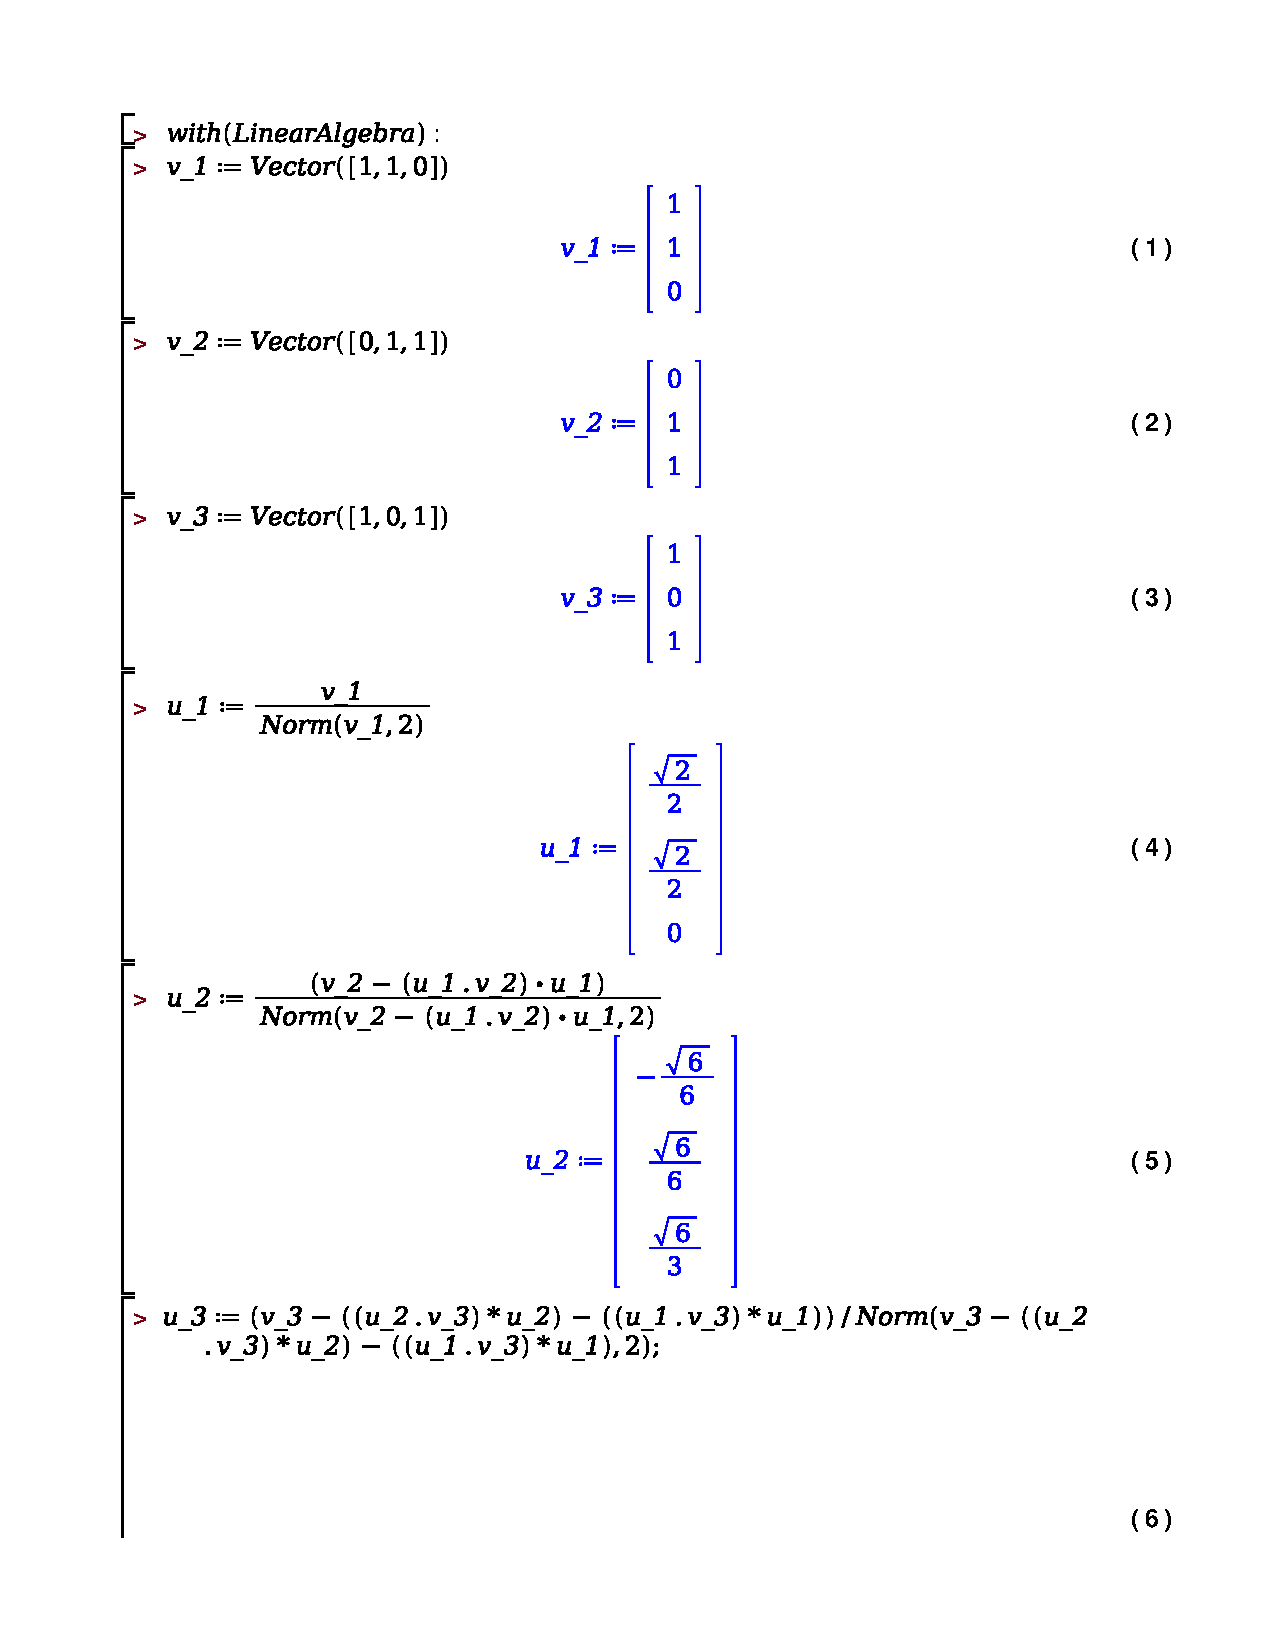
\includegraphics[width=0.8\textwidth]{./gram.pdf}
	\caption{Hier gebruiken we dus de iteratieve formule om de basis te vinden.}
	\label{fig:gramm_schmidt}
\end{figure}

\textbf{Note}: Dit kan uitgebreid worden naar functieruimtes. Hiervoor gaan we een oefening zien in het werkcollege.

\subsection{Matrices}

Typische vorm: $y=Ax$

Het \textbf{getransponeerde} is $A^T$, de rijen worden kolommen en omgekeerd.

Hier geldt dan dat: $(AB)^T = B^T A^T$, dus je draait de matrices om

\subsection{Kolomruimte, rijruimte, nulruimte}

- \textbf{Kolomruimte}: alle mogelijke lineaire combinaties van de kolommen ( $K(A)$)

- \textbf{Rijruimte}: alle mogelijke lineaire combinaties van de rijen ($K(A^T)$)

- \textbf{Nulruimte}: alle vectoren die op 0 worden afgebeeld ($N(A)$ of $N(A^T)$)

Zeer belangrijk is dat:

$N(A)$ complementair is aan $K(A^T)$ en $N(A^T)$ is complementair aan $K(A)$

Bij de representatie van het vlak heb je een \textbf{rang}. Dit is basically de hoeveelheid kolommen van $Q$ niet nul zijn.

\subsubsection{Voorbeeld definities}

Zie Figuur \ref{fig:kolom_rij_null}.

\begin{figure}[hbpt!]
	\centering
	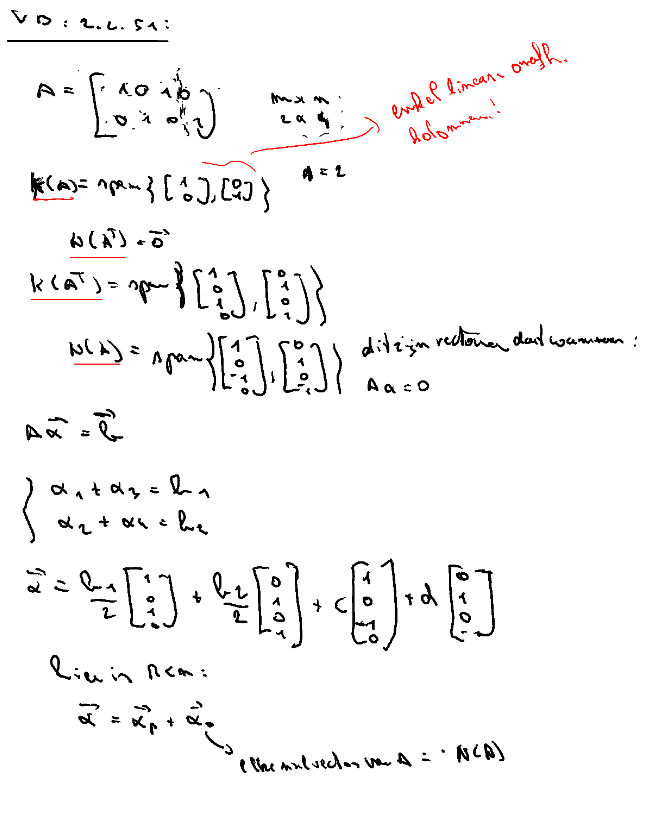
\includegraphics[width=0.8\textwidth]{assets/kolom_rij_null.png}
	\caption{}
	\label{fig:kolom_rij_null}
\end{figure}

\subsection{Matrix Inverse}

$x = A^{-1} y$

Typisch gezien is dit gedaan via: $\frac{1}{det(A)} adj(A)$

Wat heel nuttig is is dat $A A^{-1} = I$ en $A^{-1} A = I$. Dit kan heel wat schrijfwerk vermijden

Weer zoals bij transponeren geldt dat $(AB)^{-1} = B^{-1} A^{-1}$

\subsection{Projectie en kleinste kwadraten benadering}

Zoals we eerder hebben gezien bij Gramm-Schmidt, kunnen we $v= v^{||} + v^{\perp}$ schrijven.

We kunnen er iets abstracter boven plakken en werken met een \textbf{Projector}.

Deze is gedefinieerd als: $P = A (A^T A)^{-1} A^T$ (deze vorm is niet al te belangrijk).

Met de nieuwe definitie $P$ kunnen we nu zeggen dat $v = Pv + (I - P)v$

The following properties hold:

\begin{enumerate}
	\item $P^2 = P$
	\item $P^T = P$
\end{enumerate}

\subsubsection{Voorbeeld Projectie}

Zie Figuur \ref{fig:projectie}.

\begin{figure}
	\begin{center}
		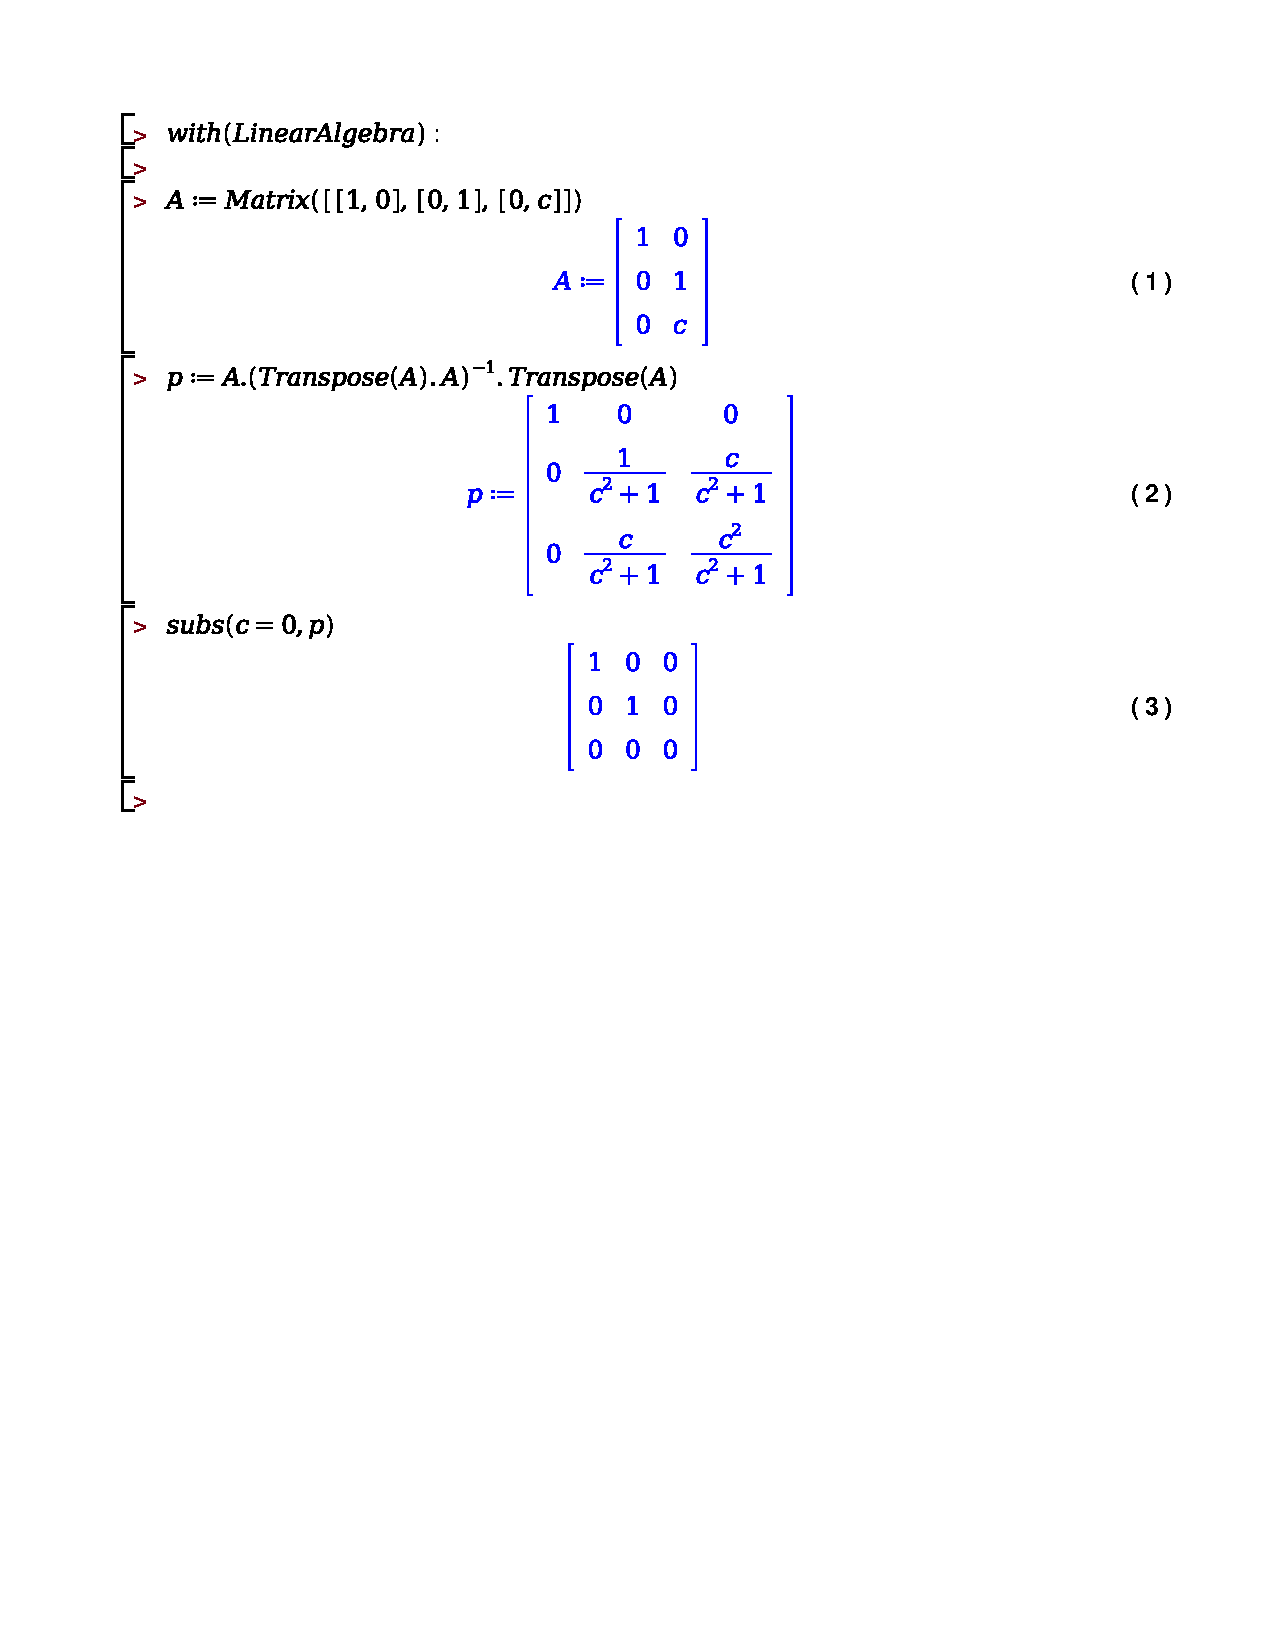
\includegraphics[width=0.95\textwidth]{./projector.pdf}
	\end{center}
	\caption{}\label{fig:projectie}
\end{figure}

\subsection{Kleinste kwadraten fit}

$x = (A^T A)^{-1} A^T y$

Dit gaat ons toelaten om te fitten op data.

In Maple wordt dit gedaan via \texttt{LinearAlgebra:-LeastSquares}.

\subsection{Vierkante matrices}

\subsubsection{Determinant}

De determinant is super handig. Hoe calculeren we deze?

Let \(\mathbf{A}\) be a \(3 \times 3\) matrix:
\[
	\mathbf{A} =
	\begin{pmatrix}
		a_{11} & a_{12} & a_{13} \\
		a_{21} & a_{22} & a_{23} \\
		a_{31} & a_{32} & a_{33}
	\end{pmatrix}
\]

The determinant of \(\mathbf{A}\), denoted as \(\det(\mathbf{A})\) or \(|\mathbf{A}|\), is calculated as:
\[
	\det(\mathbf{A}) = a_{11}(a_{22}a_{33} - a_{23}a_{32}) - a_{12}(a_{21}a_{33} - a_{23}a_{31}) + a_{13}(a_{21}a_{32} - a_{22}a_{31})
\]

Expanding the terms, we have:
\[
	\det(\mathbf{A}) = a_{11}a_{22}a_{33} - a_{11}a_{23}a_{32} - a_{12}a_{21}a_{33} + a_{12}a_{23}a_{31} + a_{13}a_{21}a_{32} - a_{13}a_{22}a_{31}
\]

Properties:

\begin{enumerate}
	\item $det(A) = det(A^T)$
	\item $det(AB) = det(A) det(B)$
	\item $det(A) = 0 -> linear dependent$
\end{enumerate}

\subsection{Basic rotation matrix}

$R(\theta) = \begin{bmatrix} cos(\theta) & -sin(\theta) \\ sin(\theta) & cos(\theta) \end{bmatrix}$

So a typical transformation equation looks like:

$\begin{bmatrix} x' \\ y' \end{bmatrix} = \begin{bmatrix} cos(\theta) & -sin(\theta) \\ sin(\theta) & cos(\theta) \end{bmatrix} \begin{bmatrix} x \\ y \end{bmatrix}$
with the middle matrix being **inverse**.

\subsubsection{Example}

See Figure \ref{fig:rotation} and \ref{fig:rotationex}.

\begin{figure}[htbp!]
	\begin{center}
		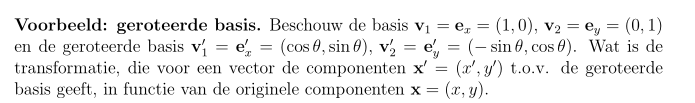
\includegraphics[width=0.7\textwidth]{./images/rotation.png}
	\end{center}
	\caption{Rotation opgave}
	\label{fig:rotation}
\end{figure}

\begin{figure}[htbp!]
	\begin{center}
		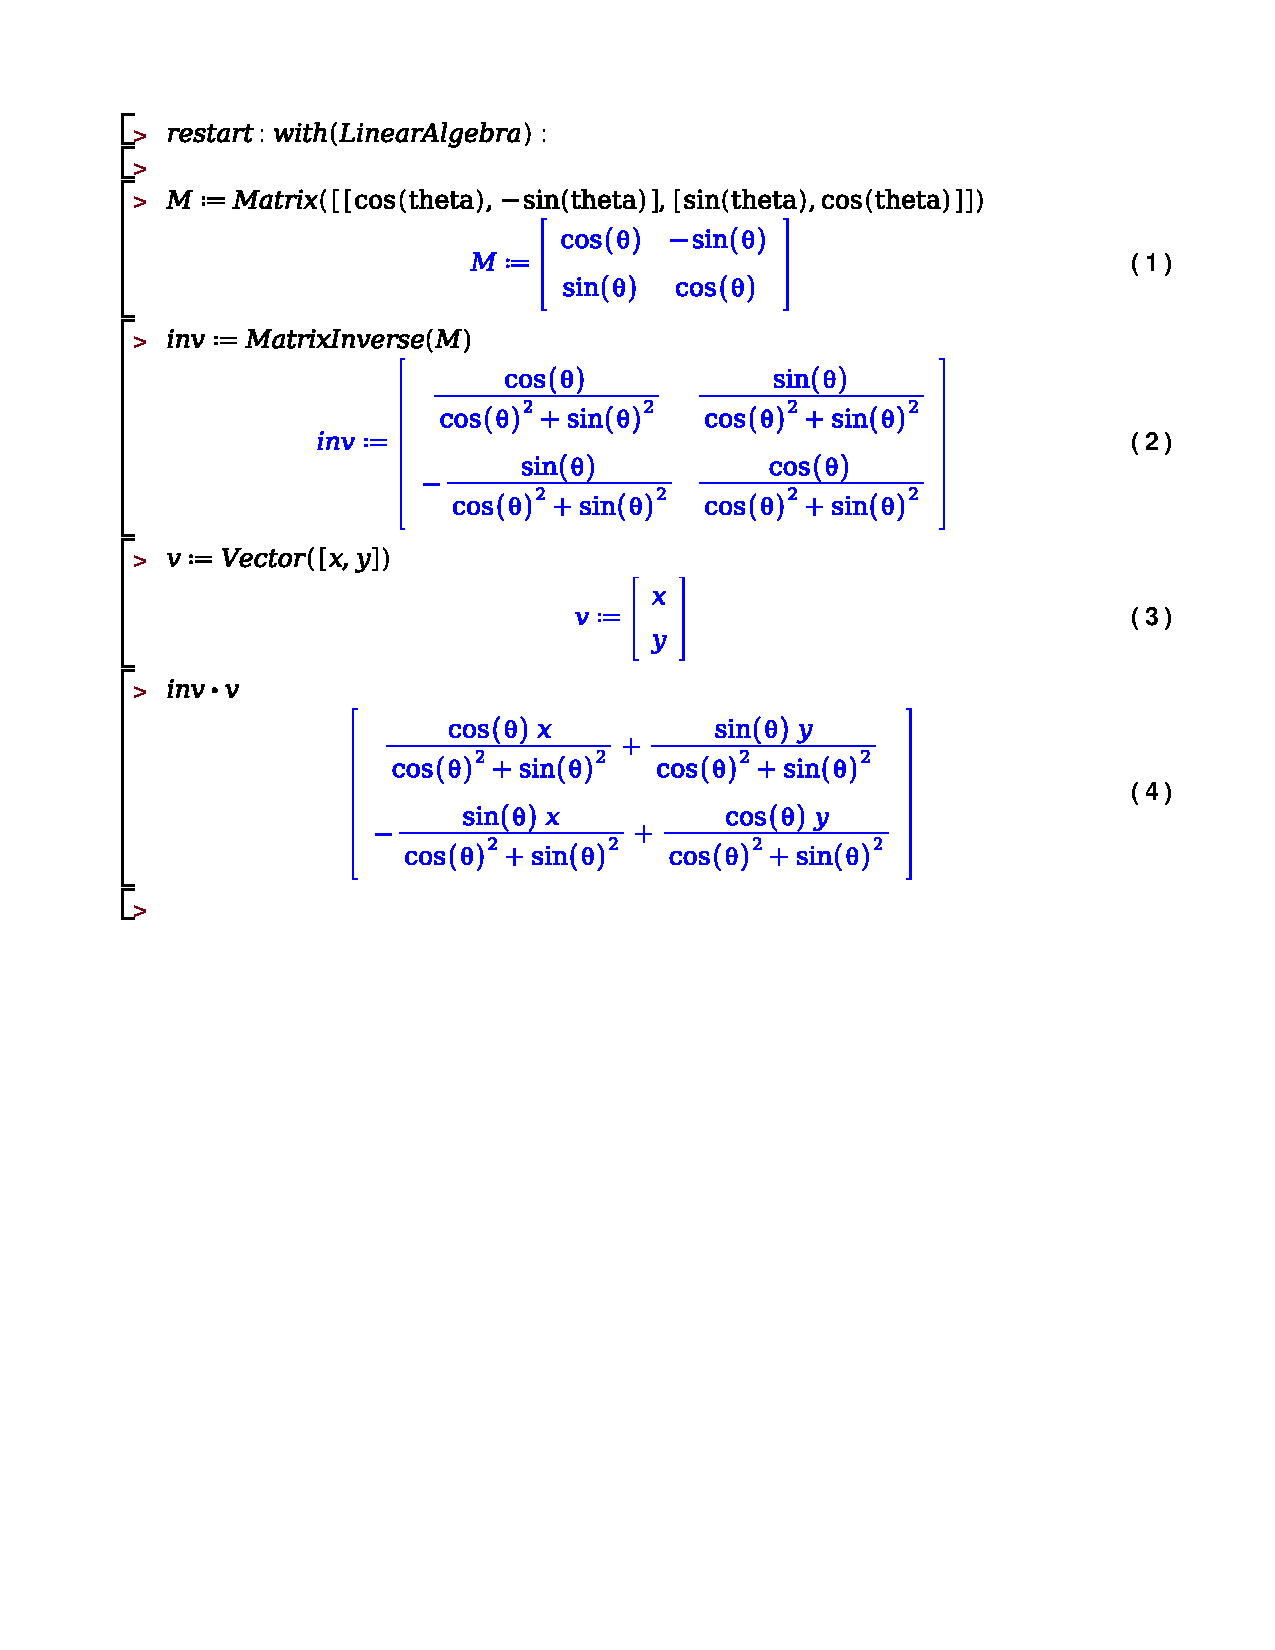
\includegraphics[width=0.7\textwidth]{./rotation.pdf}
	\end{center}
	\caption{Rotation antwoord}
	\label{fig:rotationex}
\end{figure}

\subsection{Eigenvectoren, eigenwaarden, diagonalisatie en de Jordan-decompositie}

$v_i$ is een eigenvector van A als $Av_i = \lambda_i v_i$

$p_A(\lambda) = det(A - \lambda I) = 0$

- geometrische multipliciteit: aantal lineair onafhankelijke eigenvectoren (je moet de eigenvalue invullen en row echelon reduced form verkrijgen. Dan zie je hoeveel eigenvectoren er degelijk zijn)

Figuur \ref{fig:mult} toont een voorbeeld van de multipliciteit.

\begin{figure}[htbp!]
	\begin{center}
		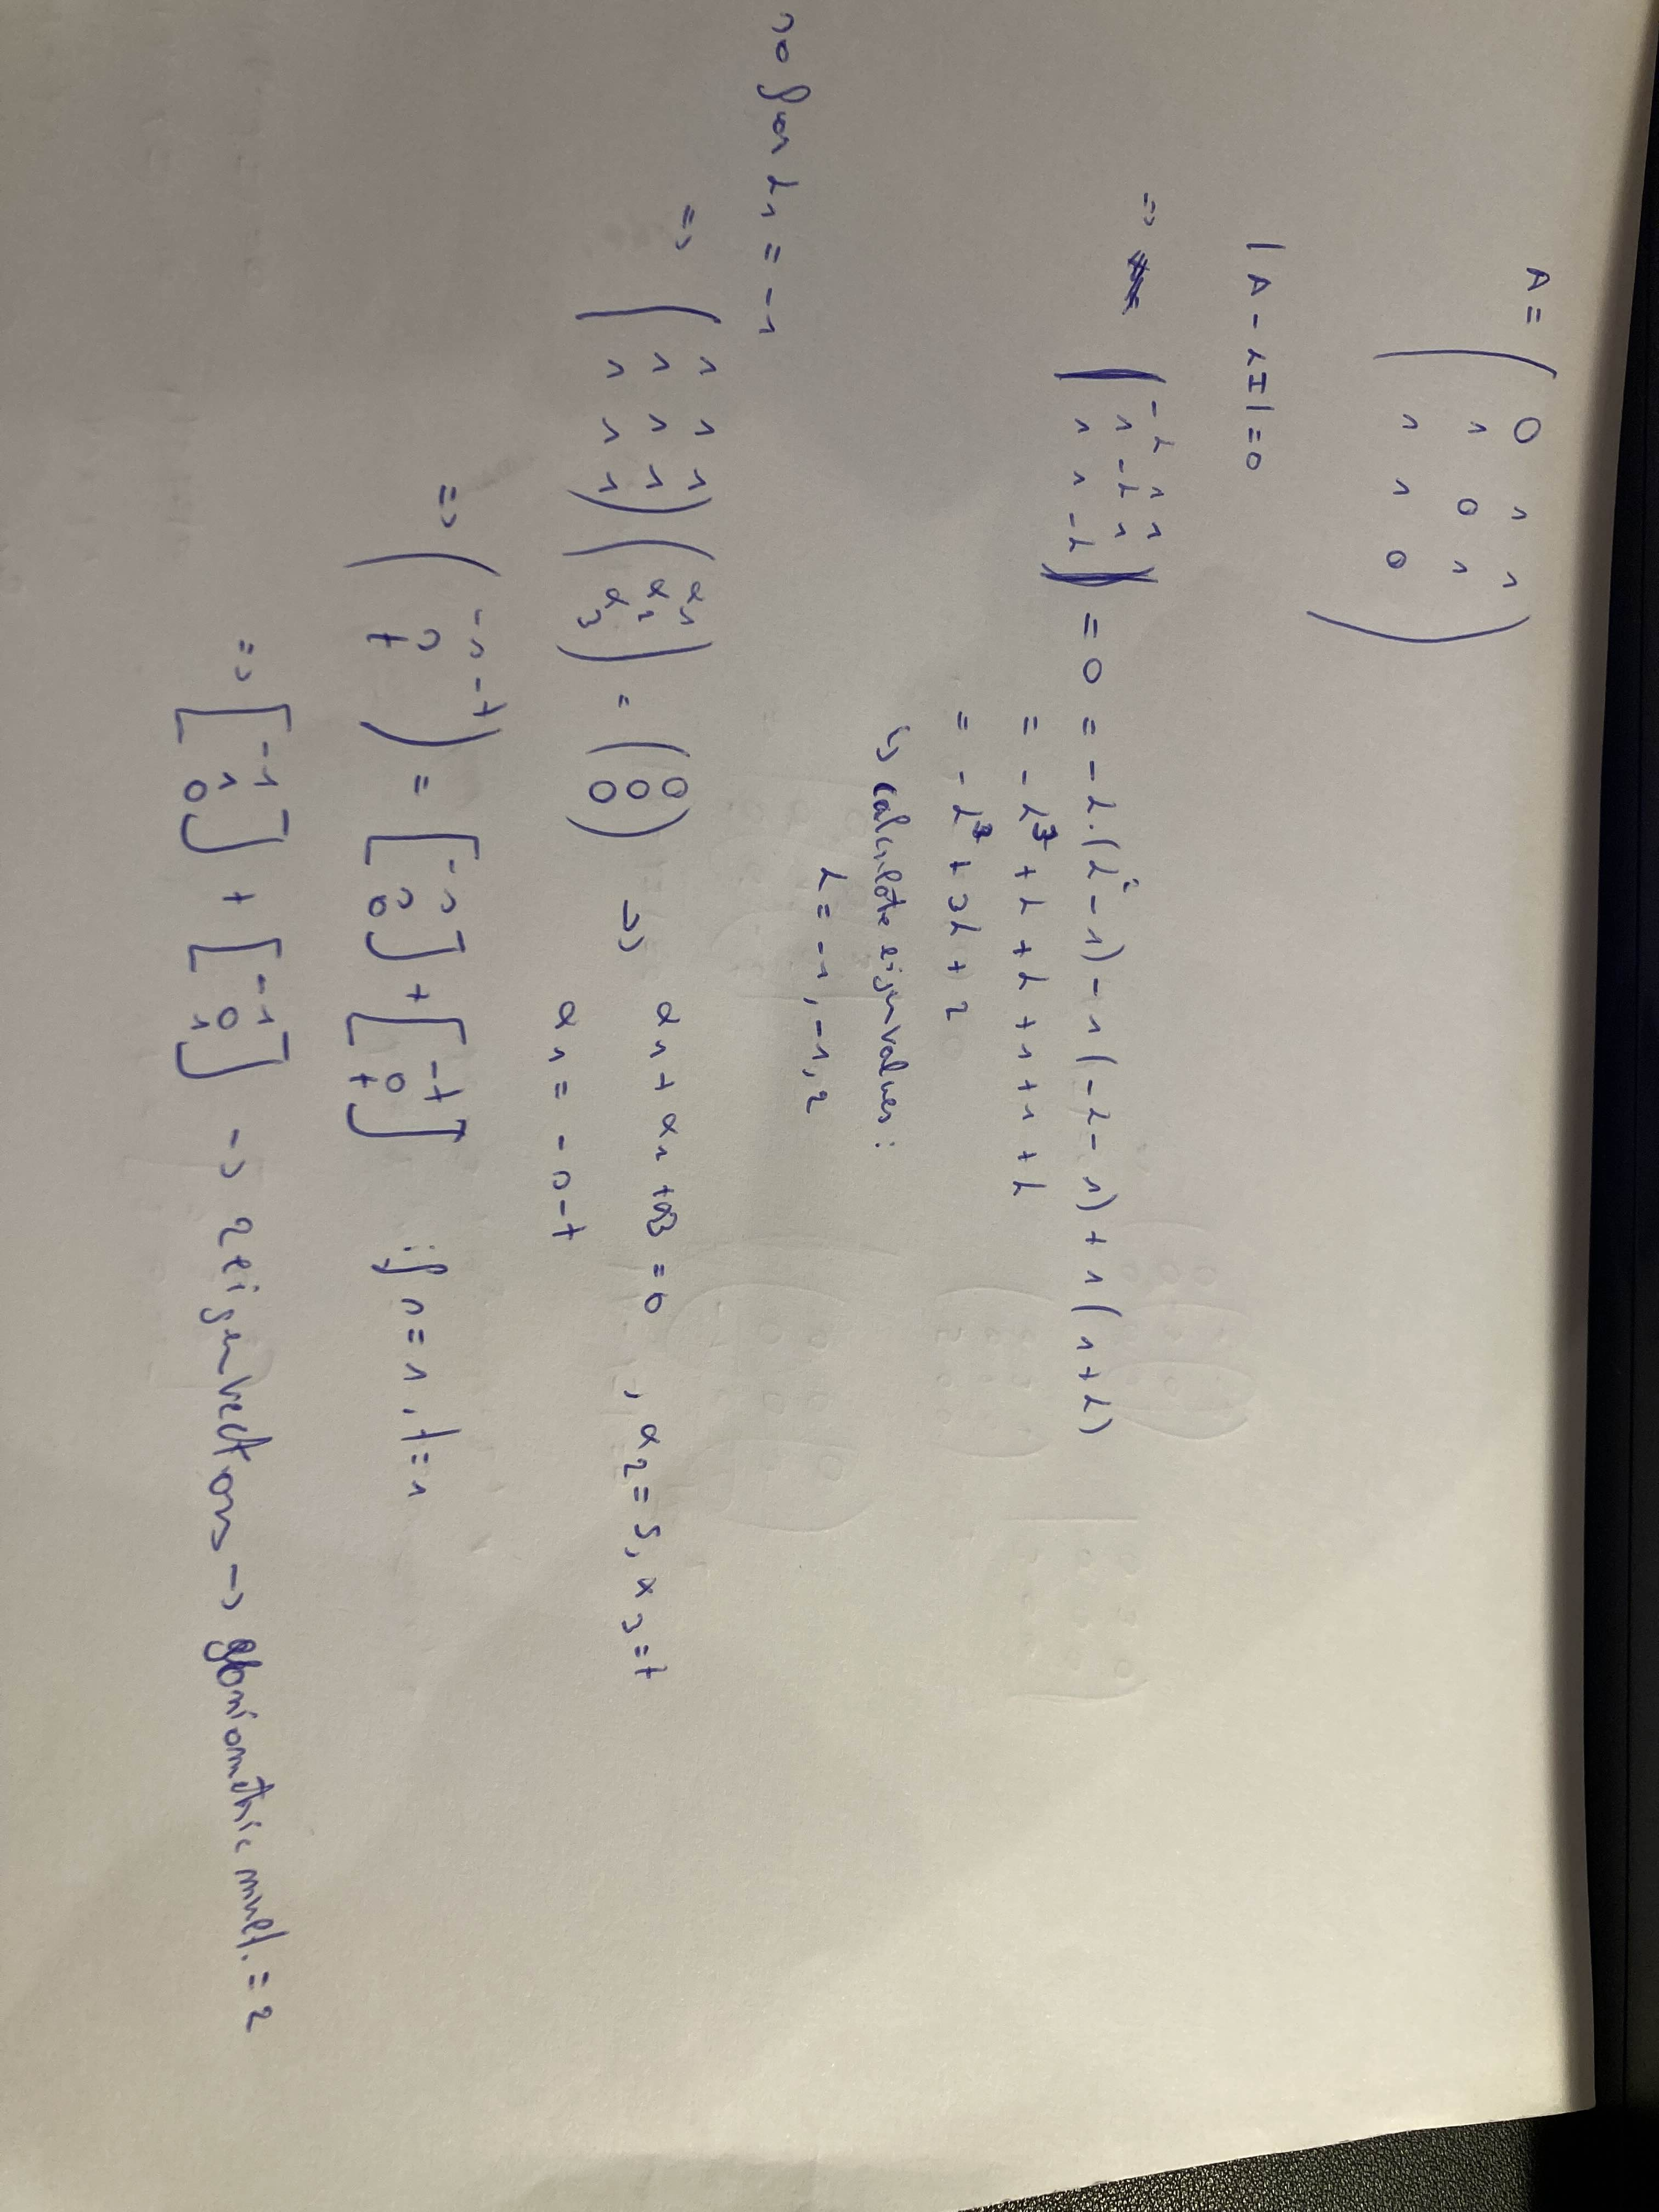
\includegraphics[width=0.95\textwidth]{./images/mult.jpg}
	\end{center}
	\caption{Een voorbeeld van de multipliciteit}
	\label{fig:mult}
\end{figure}

- algebraische multipliciteit: aantal keer dat de eigenwaarde voorkomt in de determinant

Indien alle geometrische multipliciteiten gelijk zijn aan de algebraische multipliciteiten, dan is de matrix diagonaliseerbaar.
$A = MDM^{-1}$

met $D$ een diagonale matrix met de eigenwaarden op de diagonaal.
en $M$ een matrix met de eigenvectoren.

\subsection{Jordan Form}

$A = MJM^{-1}$
met $J$ een Jordan matrix.
Dit is nodig indien de dimensie van de eigenruimte (geometrische multipliciteit) kleiner is dan de algebraische multipliciteit.
Aka, de matrix is niet diagonaliseerbaar. \ref{fig:jordan} \ref{fig:jordan_ex}

\begin{figure}[htbp!]
	\begin{center}
		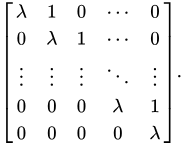
\includegraphics[width=0.95\textwidth]{./images/jordan.png}
	\end{center}
	\caption{Jordan matrix}
	\label{fig:jordan}
\end{figure}

\begin{figure}[htbp!]
	\begin{center}
		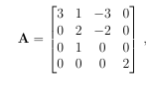
\includegraphics[width=0.95\textwidth]{./images/ex_joran.png}
	\end{center}
	\caption{Jordan matrix example}
	\label{fig:jordan_ex}
\end{figure}

This gives us: \ref{fig:jordan_sol}

\begin{figure}[htbp!]
	\begin{center}
		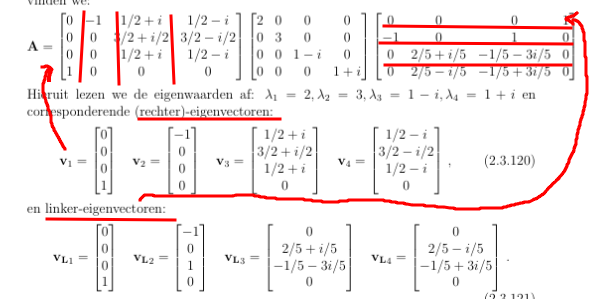
\includegraphics[width=0.95\textwidth]{./images/sol_jordan.png}
	\end{center}
	\caption{Jordan matrix solution}
	\label{fig:jordan_sol}
\end{figure}

\subsubsection{Example}

See Figure \ref{fig:jordan_ex_2}.
\begin{figure}[htbp!]
	\begin{center}
		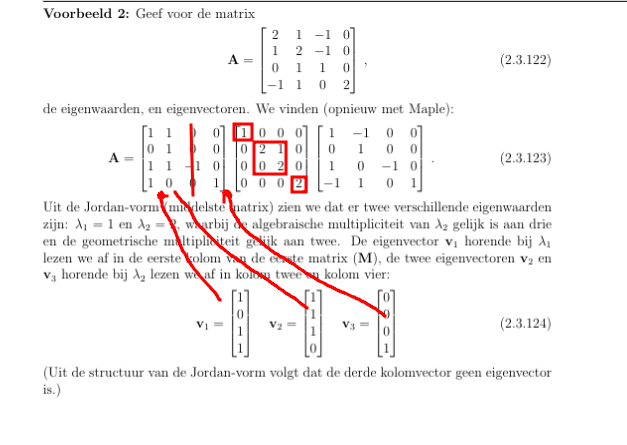
\includegraphics[width=0.95\textwidth]{./images/jordan_ex_2.png}
	\end{center}
	\caption{Jordan matrix example 2}
	\label{fig:jordan_ex_2}
\end{figure}

\subsection{Matrixmachten en iteratieve matrixvergelijkingen}

$A^k = M D^k M^{-1}$ voor diagonaliseerbare matrices

$A^k = M J^k M^{-1}$ voor niet-diagonaliseerbare matrices

met diagonaal matrix: \ref{fig:diag}

\begin{figure}[htbp!]
	\begin{center}
		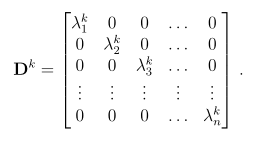
\includegraphics[width=0.95\textwidth]{./images/diag.png}
	\end{center}
	\caption{Diagonaal matrix}
	\label{fig:diag}
\end{figure}

\textbf{iteratieve matrixvergelijking}: $x_k = M D^k M^{-1} x_0$ Op deze manier kun je telkens de $k_{de}$ stap berekenen.

Dit is enkel voor de diagonaliseerbare matrices. ($A^k = M D^k M^{-1}$)

\textbf{asymptotisch gedrag}: $\lim_{k \to \infty} u_k = \lambda^k (v_{L1} * u_0) v_1$

$v_1$ is een fixed point in het asymptotisch gedrag.

\subsubsection{Voorbeeld}

Zie Figuur \ref{fig:fibo}.

\begin{figure}[htbp!]
	\begin{center}
		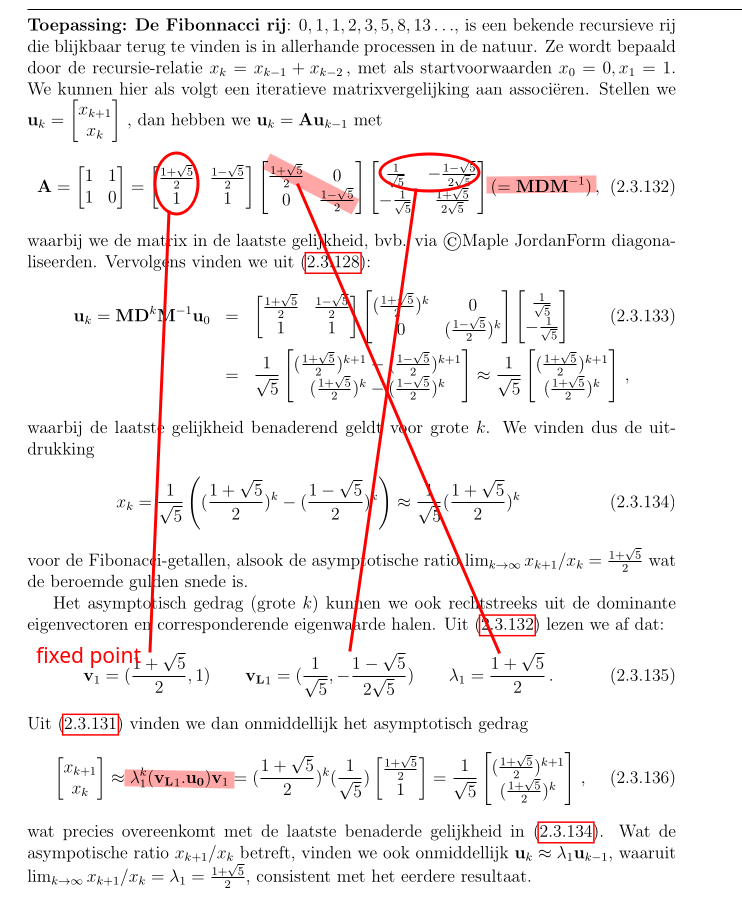
\includegraphics[width=0.95\textwidth]{./images/fibo.png}
	\end{center}
	\caption{Fibonacci voorbeeld}
	\label{fig:fibo}
\end{figure}

In het bovenstaande zien we dat $\lambda_1$ de dominante eigenwaarde is. Daardoor kunnen we de fixed point berekenen met:

$\lambda_1^k (v_{L1} . u_0) v_1$

Omdat $\lambda_1$ dominant is, nemen we voor $v_1$ de eerste kolom van $M$ en voor $v_{L1}$ de eerste rij van $M^{-1}$

Dit kan toegepast worden in de zogezegde \textbf{Markov proces}

algemene vorm: $u_k = P u_{k - 1}$
waarbij $P$ een matrix is die de overgangen tussen de verschillende states aangeeft met probabiliteit.
$\sum p_{ij} = 1$

Ook goed om te weten is dat wanneer de matrix strikt positieve getallen heeft, dat matrix $P$ een uniek dominante eigenwaarde $\lambda_1 = 1$ heeft met $v_1$ een positieve eigenvector. Deze $v_1$ is dan ook een fixed point.

\subsubsection{Voorbeeld Markov proces}

Zie Figuur \ref{fig:markov} and \ref{fig:markovsol}.

\begin{figure}[htbp!]
	\begin{center}
		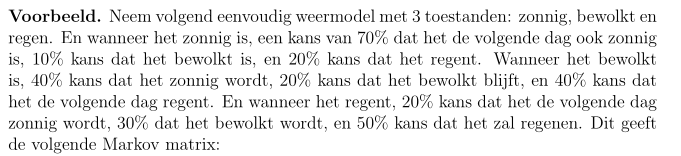
\includegraphics[width=0.95\textwidth]{./images/markov.png}
	\end{center}
	\caption{Markov proces}
	\label{fig:markov}

\end{figure}
\begin{figure}[htbp!]
	\begin{center}
		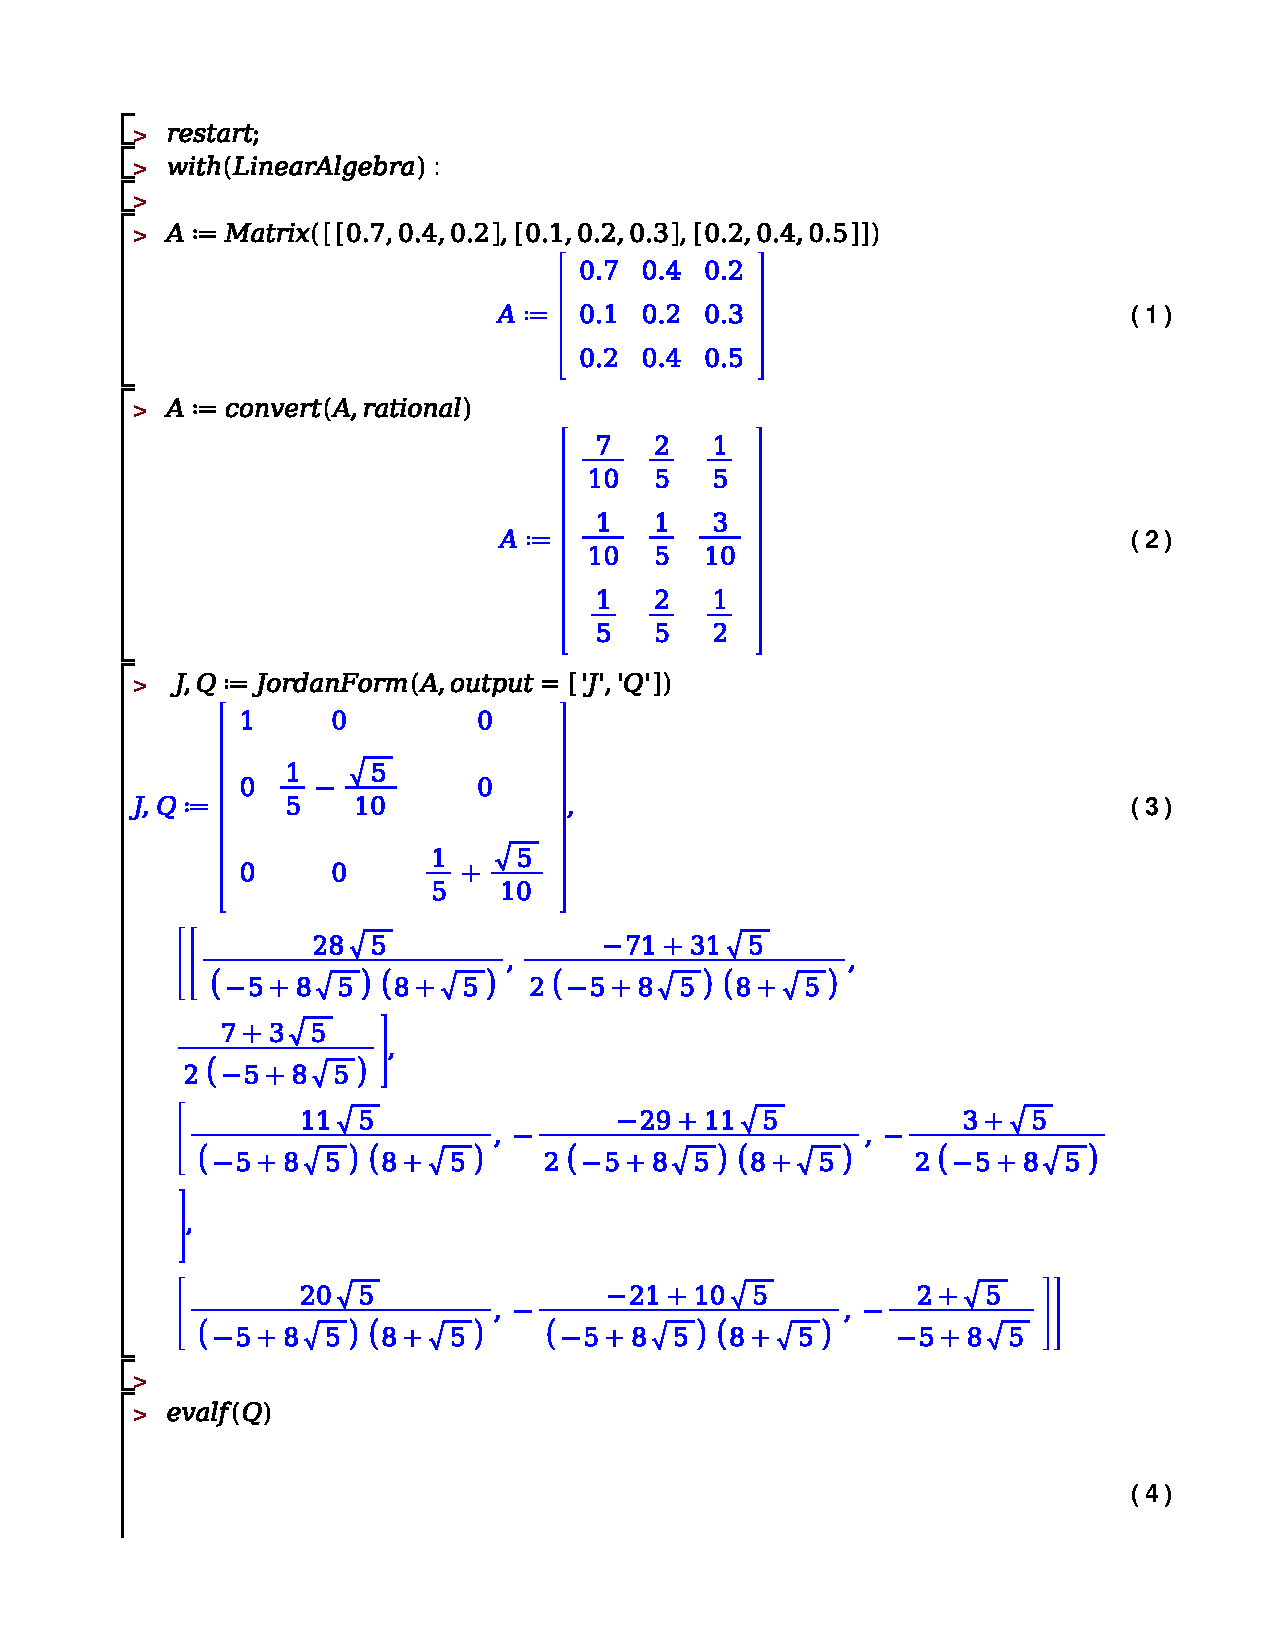
\includegraphics[width=0.95\textwidth]{./markov.pdf}
	\end{center}
	\caption{Markov proces solution}
	\label{fig:markovsol}
\end{figure}

\subsection{Matrixexponent en lineaire differentiaalvergelijkingen}

Hier gaan we een matrix plaatsen de exponent.

$e^{At} = M e^{Dt} M^{-1}$ -> concreet voorbeeld

\textbf{Algemeen}:

$e^{A} = \sum_{k=0}^{\infty} \frac{A^k}{k!}$

of

$e^{A} = M e^{D} M^{-1}$ || $e^{A} = M e^{J} M^{-1}$ (niet-diagonaliseerbare matrices)

In matrix vorm zie je het volgende: \ref{fig:matrix_expo}

\begin{figure}[htbp!]
	\begin{center}
		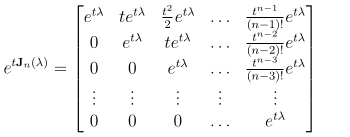
\includegraphics[width=0.95\textwidth]{./images/matrix_expo.png}
	\end{center}
	\caption{Matrix exponent}
	\label{fig:matrix_expo}
\end{figure}

Note: Maple geeft de functie `MatrixExponential(A, t)` om $e^{At}$ te berekenen.

\subsubsection{eerste-orde differentiaalvergelijking}

$y'(t) = Ay(t)$

$y(t) = e^{At} y(0)$

\subsubsection{n-de differentiaalvergelijkin}

Hetzelfde als hierboven

\subsubsection{Herschrijf de tweede-orde differentiaalvergelijking $y''(t) + w^2 y(t) = 0$}

Zie Figuur \ref{fig:diff2}.

\begin{figure}[htbp!]
	\begin{center}
		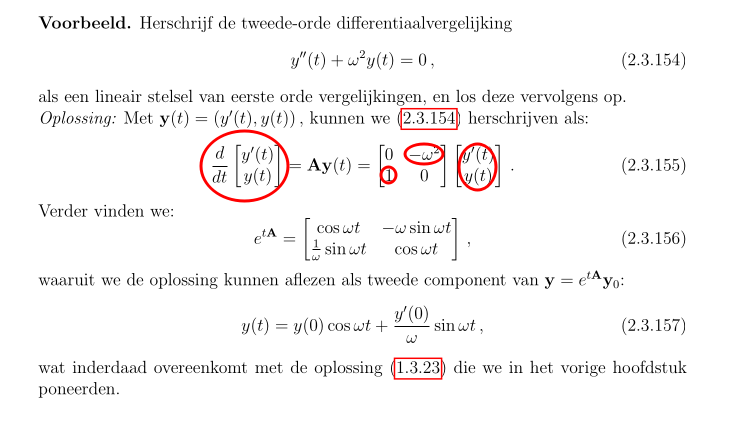
\includegraphics[width=0.95\textwidth]{./images/something.png}
	\end{center}
	\caption{Tweede-orde differentiaalvergelijking}
	\label{fig:diff2}
\end{figure}

\subsection{Symmetrische matrices}

- $A = A^T$
- $A$ heeft enkel reele eigenwaarden
- $A$ heeft orthogonale eigenvectoren
- $A = ODO^T$ met $O$ een orthogonale matrix en $D$ een diagonale matrix

Omdat $O^T = O^{-1}$, kunnen we zeggen dat $O^T O = I$

Ook is het zo dat geometrische multipliciteit = algebraische multipliciteit. -> $A$ is diagonaliseerbaar.

\subsection{SVD (Singular Value Decomposition)}

$A = U \Sigma V^T$

of

$A = \sum_{i=1}^{r} \sigma_i u_i v_i^T$


met $U$ en $V$ orthogonale matrices en $\Sigma$ een diagonale matrix met singular values

$U$ is mxm, $V$ is nxn en $\Sigma$ is mxn


\subsubsection{Example SVD}

Als we compressie willen uitvoeren moeten we essentially SVD uitvoeren, maar onze som wordt beperkt door een rang $r'$

$A = \sum_{i=1}^{r'} \sigma_i u_i v_i^T$

\chapter{Hoofdstuk 3: Integratie en afleiding in $R^n$}

\subsection{Partiele afgeleiden}

$D_i f(x_1, x_2, ... x_n) = \frac{\partial f}{\partial x_i}$

\subsubsection{Example}

\begin{figure}[H]
	\begin{center}
		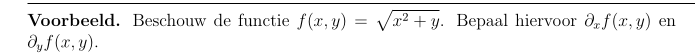
\includegraphics[width=0.95\textwidth]{./images/partial.png}
	\end{center}
	\caption{Partial derivatives example}
	\label{}
\end{figure}
\begin{figure}[H]
	\begin{center}
		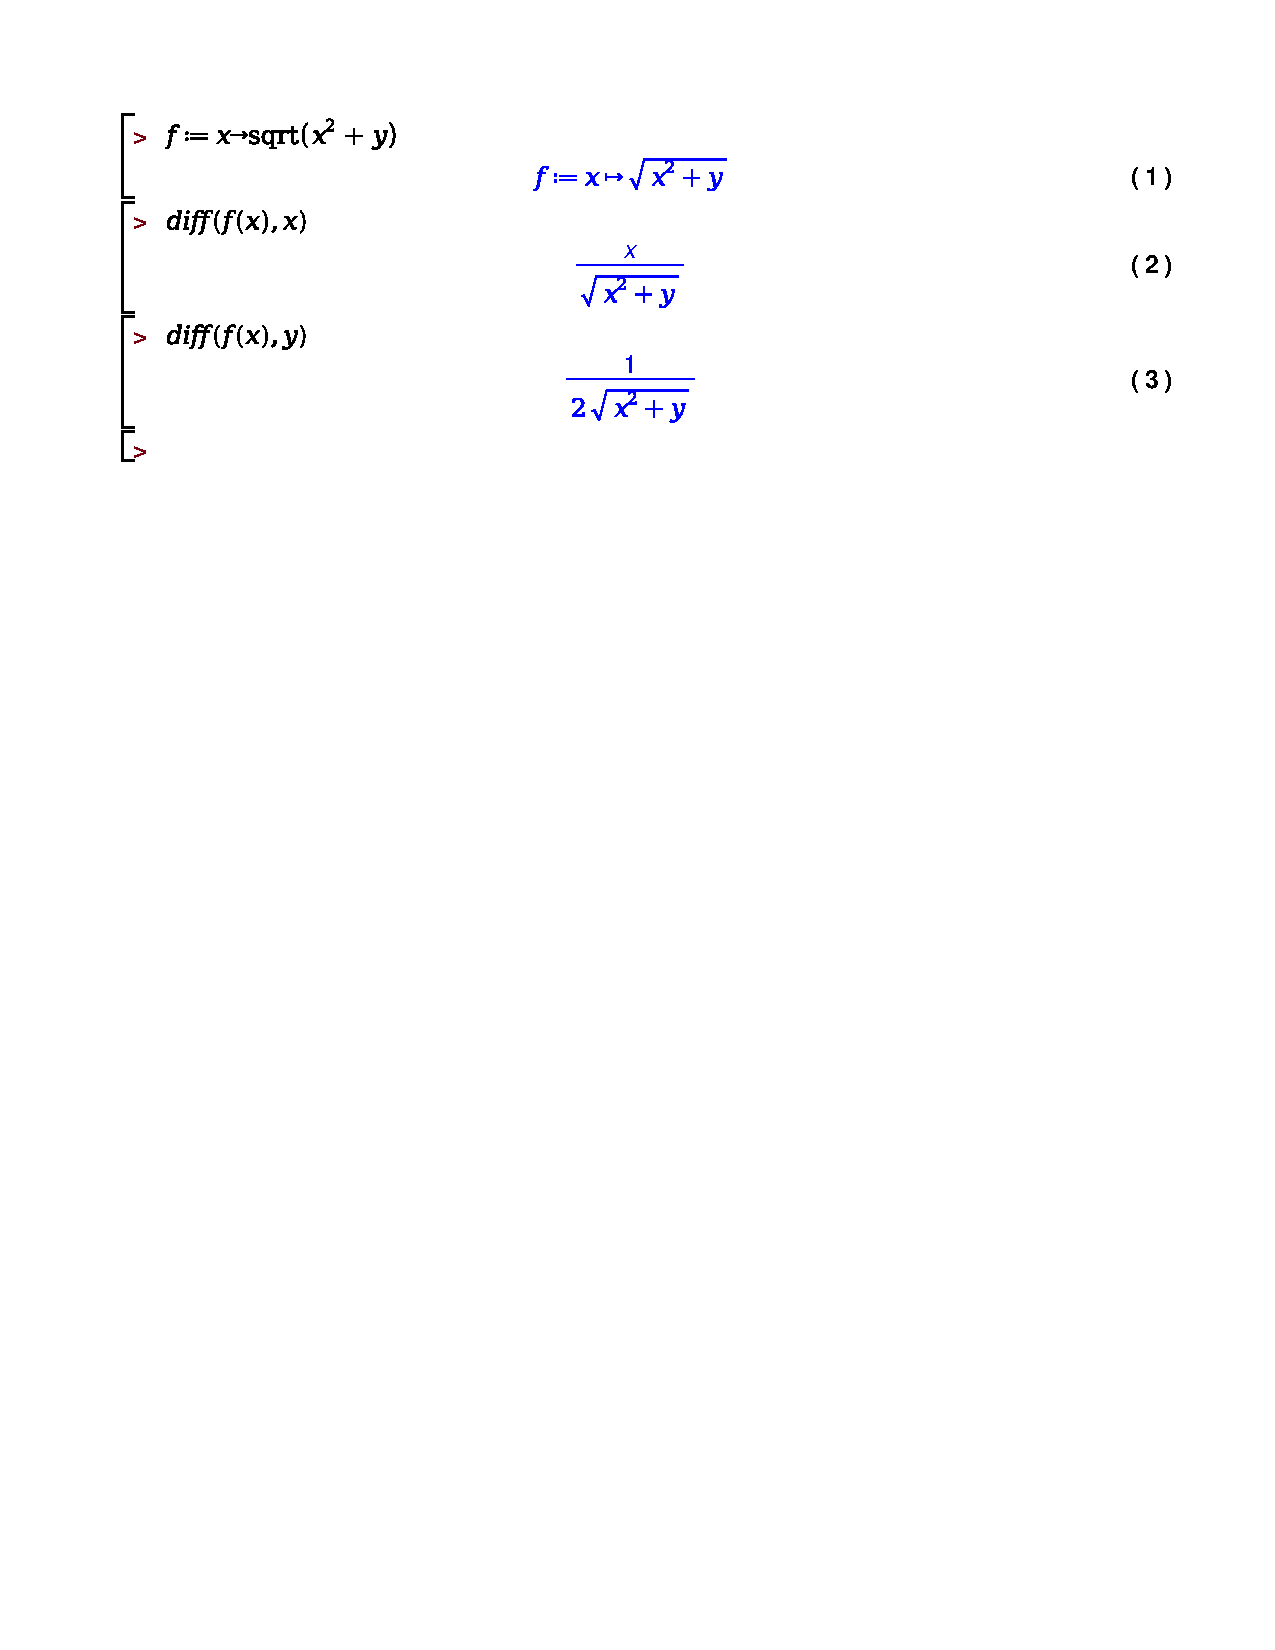
\includegraphics[width=0.95\textwidth]{./partial.pdf}
	\end{center}
	\caption{Partial derivatives example}
	\label{}
\end{figure}

\textbf{Higher order partial derivatives}:

Basically hetzelfde, doe het gewoon na elkaar, van binnen naar buiten

\begin{figure}[H]
	\begin{center}
		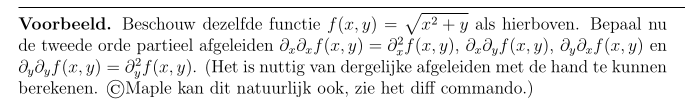
\includegraphics[width=0.95\textwidth]{./images/partial_2.png}
	\end{center}
	\caption{Partial derivatives example}
	\label{}
\end{figure}

\begin{figure}[H]
	\begin{center}
		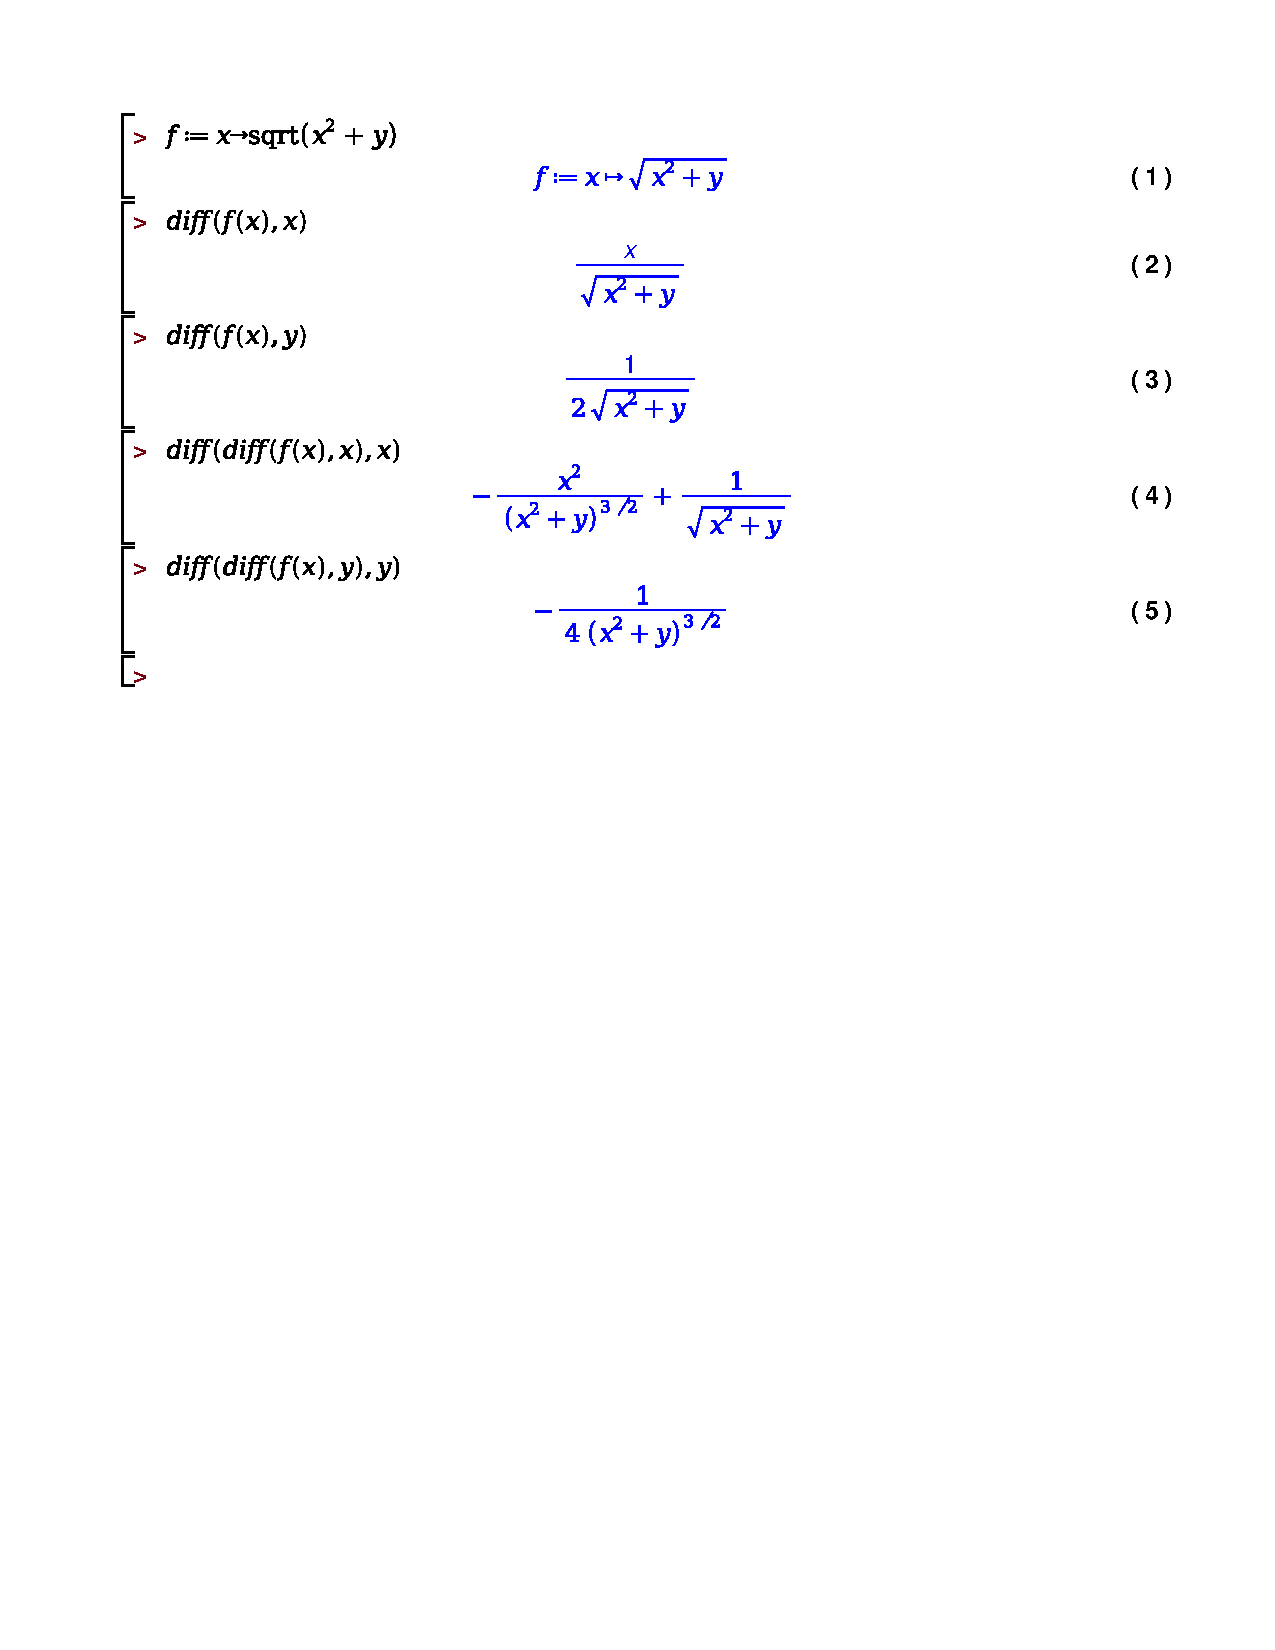
\includegraphics[width=0.95\textwidth]{./partial_2.pdf}
	\end{center}
	\caption{Partial derivatives example}
	\label{}
\end{figure}

\subsection{Kettingregel}

When deriving, make sure to derive the respected variable as well.

\subsection{Coordinaten transformaties}

Hier gaan we de coordinaten transformeren naar een andere coordinatenstelsel. (om het probleem zo gemakkelijk mogelijk te maken)

\subsubsection{Example}

\begin{figure}[H]
	\begin{center}
		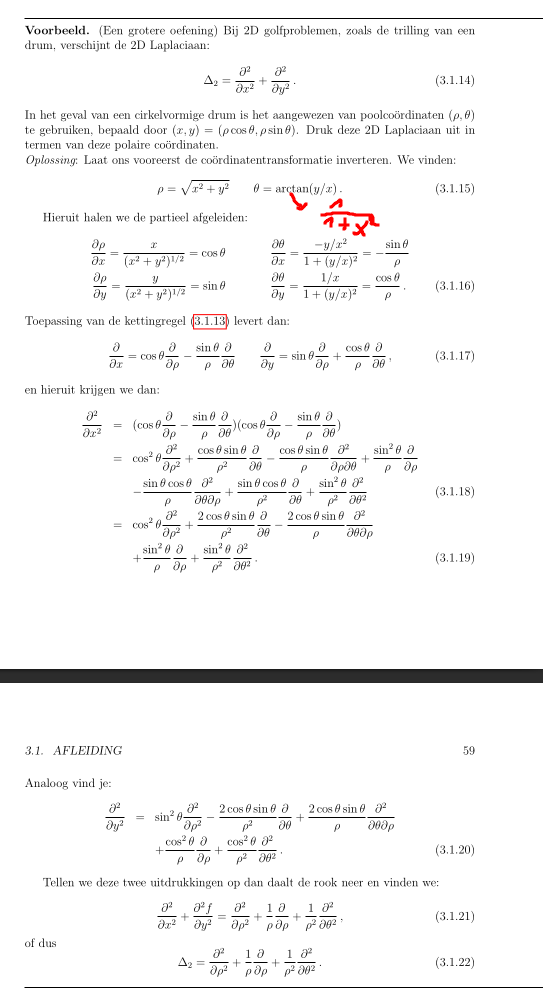
\includegraphics[width=0.95\textwidth]{./images/coordinaten.png}
	\end{center}
	\caption{Coordinaten transformaties}
	\label{}
\end{figure}

1. Calculeer de $\rho$ en $\theta$ naar x en y

2. vorm de chain rule: $\frac{\partial}{\partial x} = \frac{\partial \rho}{\partial x} \frac{\partial}{\partial \rho} + \frac{\partial \theta}{\partial x} \frac{\partial}{\partial \theta}$

3. doe hetzelfde voor met respect tot y.

4. Vermenigvuldig twee maal met elkaar door de dubbele afgeleide

5. som met elkaar

6. Je hebt nu de laplacian ($\nabla^2 f = \frac{\partial^2 f}{\partial x^2} + \frac{\partial^2 f}{\partial y^2} + \frac{\partial^2 f}{\partial z^2}$)

\subsection{Gradient en de differentiaal}

\textbf{gradient operator}: $\nabla = \sum_{i=1}^{n} e_i \partial_i$

Via deze gradient kunnen we de richtingsafgeleide berekenen (variatie van een functie langs een kromme)

$\nabla f . \frac{dx}{dt}$

\subsubsection{Example}

\begin{figure}[H]
	\begin{center}
		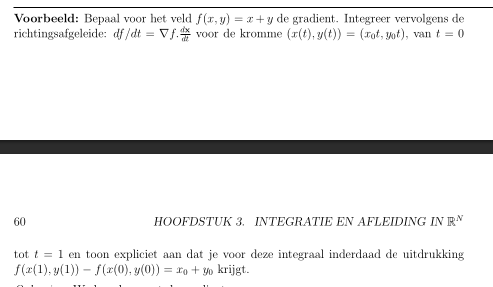
\includegraphics[width=0.95\textwidth]{./images/gradient.png}
	\end{center}
	\caption{Gradient example}
	\label{}
\end{figure}

Hier zien we dat de gradient $\nabla = (\partial_x, \partial_y)$ = (1, 1) (want f(x, y) = x + y)

de richtingsafgeleide is dan $\nabla f . \frac{dx}{dt} = (1, 1) . (x_0, y_0) = x_0 + y_0$

Als je de integraal pakt van t = 0 naar t = 1: $\int_0^1 x_0 + y_0 dt = x_0 + y_0$

De gradient operator en richtingsafgeleide wordt gebruikt bij zaken zoals stochastic gradient descent, waar we proberen de lokale minima te vinden.

\subsubsection{Example}
\begin{figure}[H]
	\begin{center}
		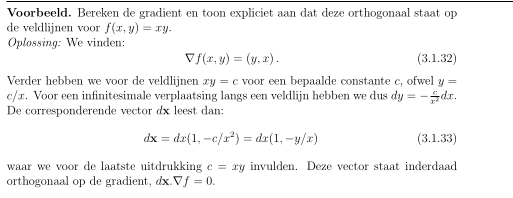
\includegraphics[width=0.95\textwidth]{./images/gradient_2.png}
	\end{center}
	\caption{Gradient example}
	\label{}
\end{figure}

1. Calculate the gradient

$\nabla f = (\partial_x, \partial_y) = (y, x)$

onze veldijn: $c = xy$
Note: We willen uiteindelijk kunnen zeggen dat onze richtingsafgeleide = 0, we hebben dus \textbf{dx} nodig

$y = \frac{c}{x}$

$dy = - \frac{c}{x^2} dx$

We weten ook dat onze displacement along the kromme $dx = (dx, dy)$

We weten nu wel $dy$ dus we vullen dit in: $dx = (dx, - \frac{c}{x^2} dx) = dx(1, - \frac{c}{x^2})$

We weten ook wat c is: $dx(1, - \frac{xy}{x^2}) = dx(1, - \frac{y}{x})$

Nu dat we de displacement hebben, vinden we de richtingsafgeleide:

$\nabla f . dx = (y, x) . dx(1, - \frac{y}{x}) = ydx - ydx = 0$

Dus hebben we bewezen dat de gradient $\nabla f$ loodrecht staat op de kromme.

\subsection{Taylorreeks}

\begin{figure}[H]
	\begin{center}
		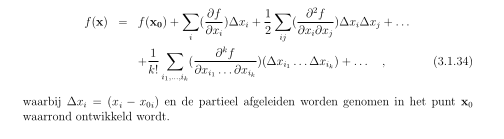
\includegraphics[width=0.95\textwidth]{./images/taylor_afgeleid.png}
	\end{center}
	\caption{Taylorreeks bij afgeleiden}
	\label{}
\end{figure}

Als $\triangle_{xi}$ (tweede term van taylorreeks), we $\nabla f . \triangle_{xi}$

Dit is een \textbf{stationair punt} wanneer $\nabla f = 0$

Er zijn hierbij 3 gevallen voor 1 variable:

- $\frac{\partial^2 f}{\partial x_i^2} > 0$ (minimum)

- $\frac{\partial^2 f}{\partial x_i^2} < 0$ (maximum)

- $\frac{\partial^2 f}{\partial x_i^2} = 0$ (saddle point (stationair buigpunt))

Voor meerdere variablen, maken we gebruik van de \textbf{Hessiaan} dat voorkomt in de tweede orde term van de taylorreeks:

- Hessiaan is symmetrisch, dus $H = O D O^T$

\begin{figure}[H]
	\begin{center}
		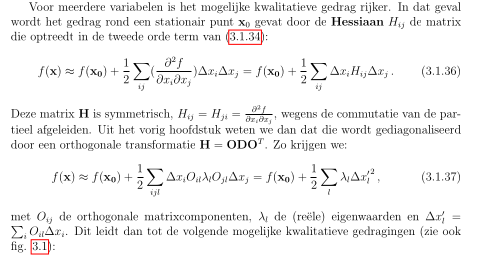
\includegraphics[width=0.95\textwidth]{./images/hessiaan.png}
	\end{center}
	\caption{Hessiaan}
	\label{}
\end{figure}

- als alle $\lambda_i > 0$ (minimum)

- als alle $\lambda_i < 0$ (maximum)

- als er zowel positieve als negatieve $\lambda_i$ zijn (saddle point)

- als er eigenwaarden zijn die = 0, dan krijg je in sommige richtingen een stationair buigpunt gedefinieerd door de derde orde vorm van taylorreeks

\subsubsection{Example}

\begin{figure}[H]
	\begin{center}
		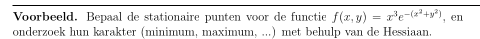
\includegraphics[width=0.95\textwidth]{./images/hessian_ex.png}
	\end{center}
	\caption{Hessiaan}
	\label{}
\end{figure}

\begin{figure}[H]
	\begin{center}
		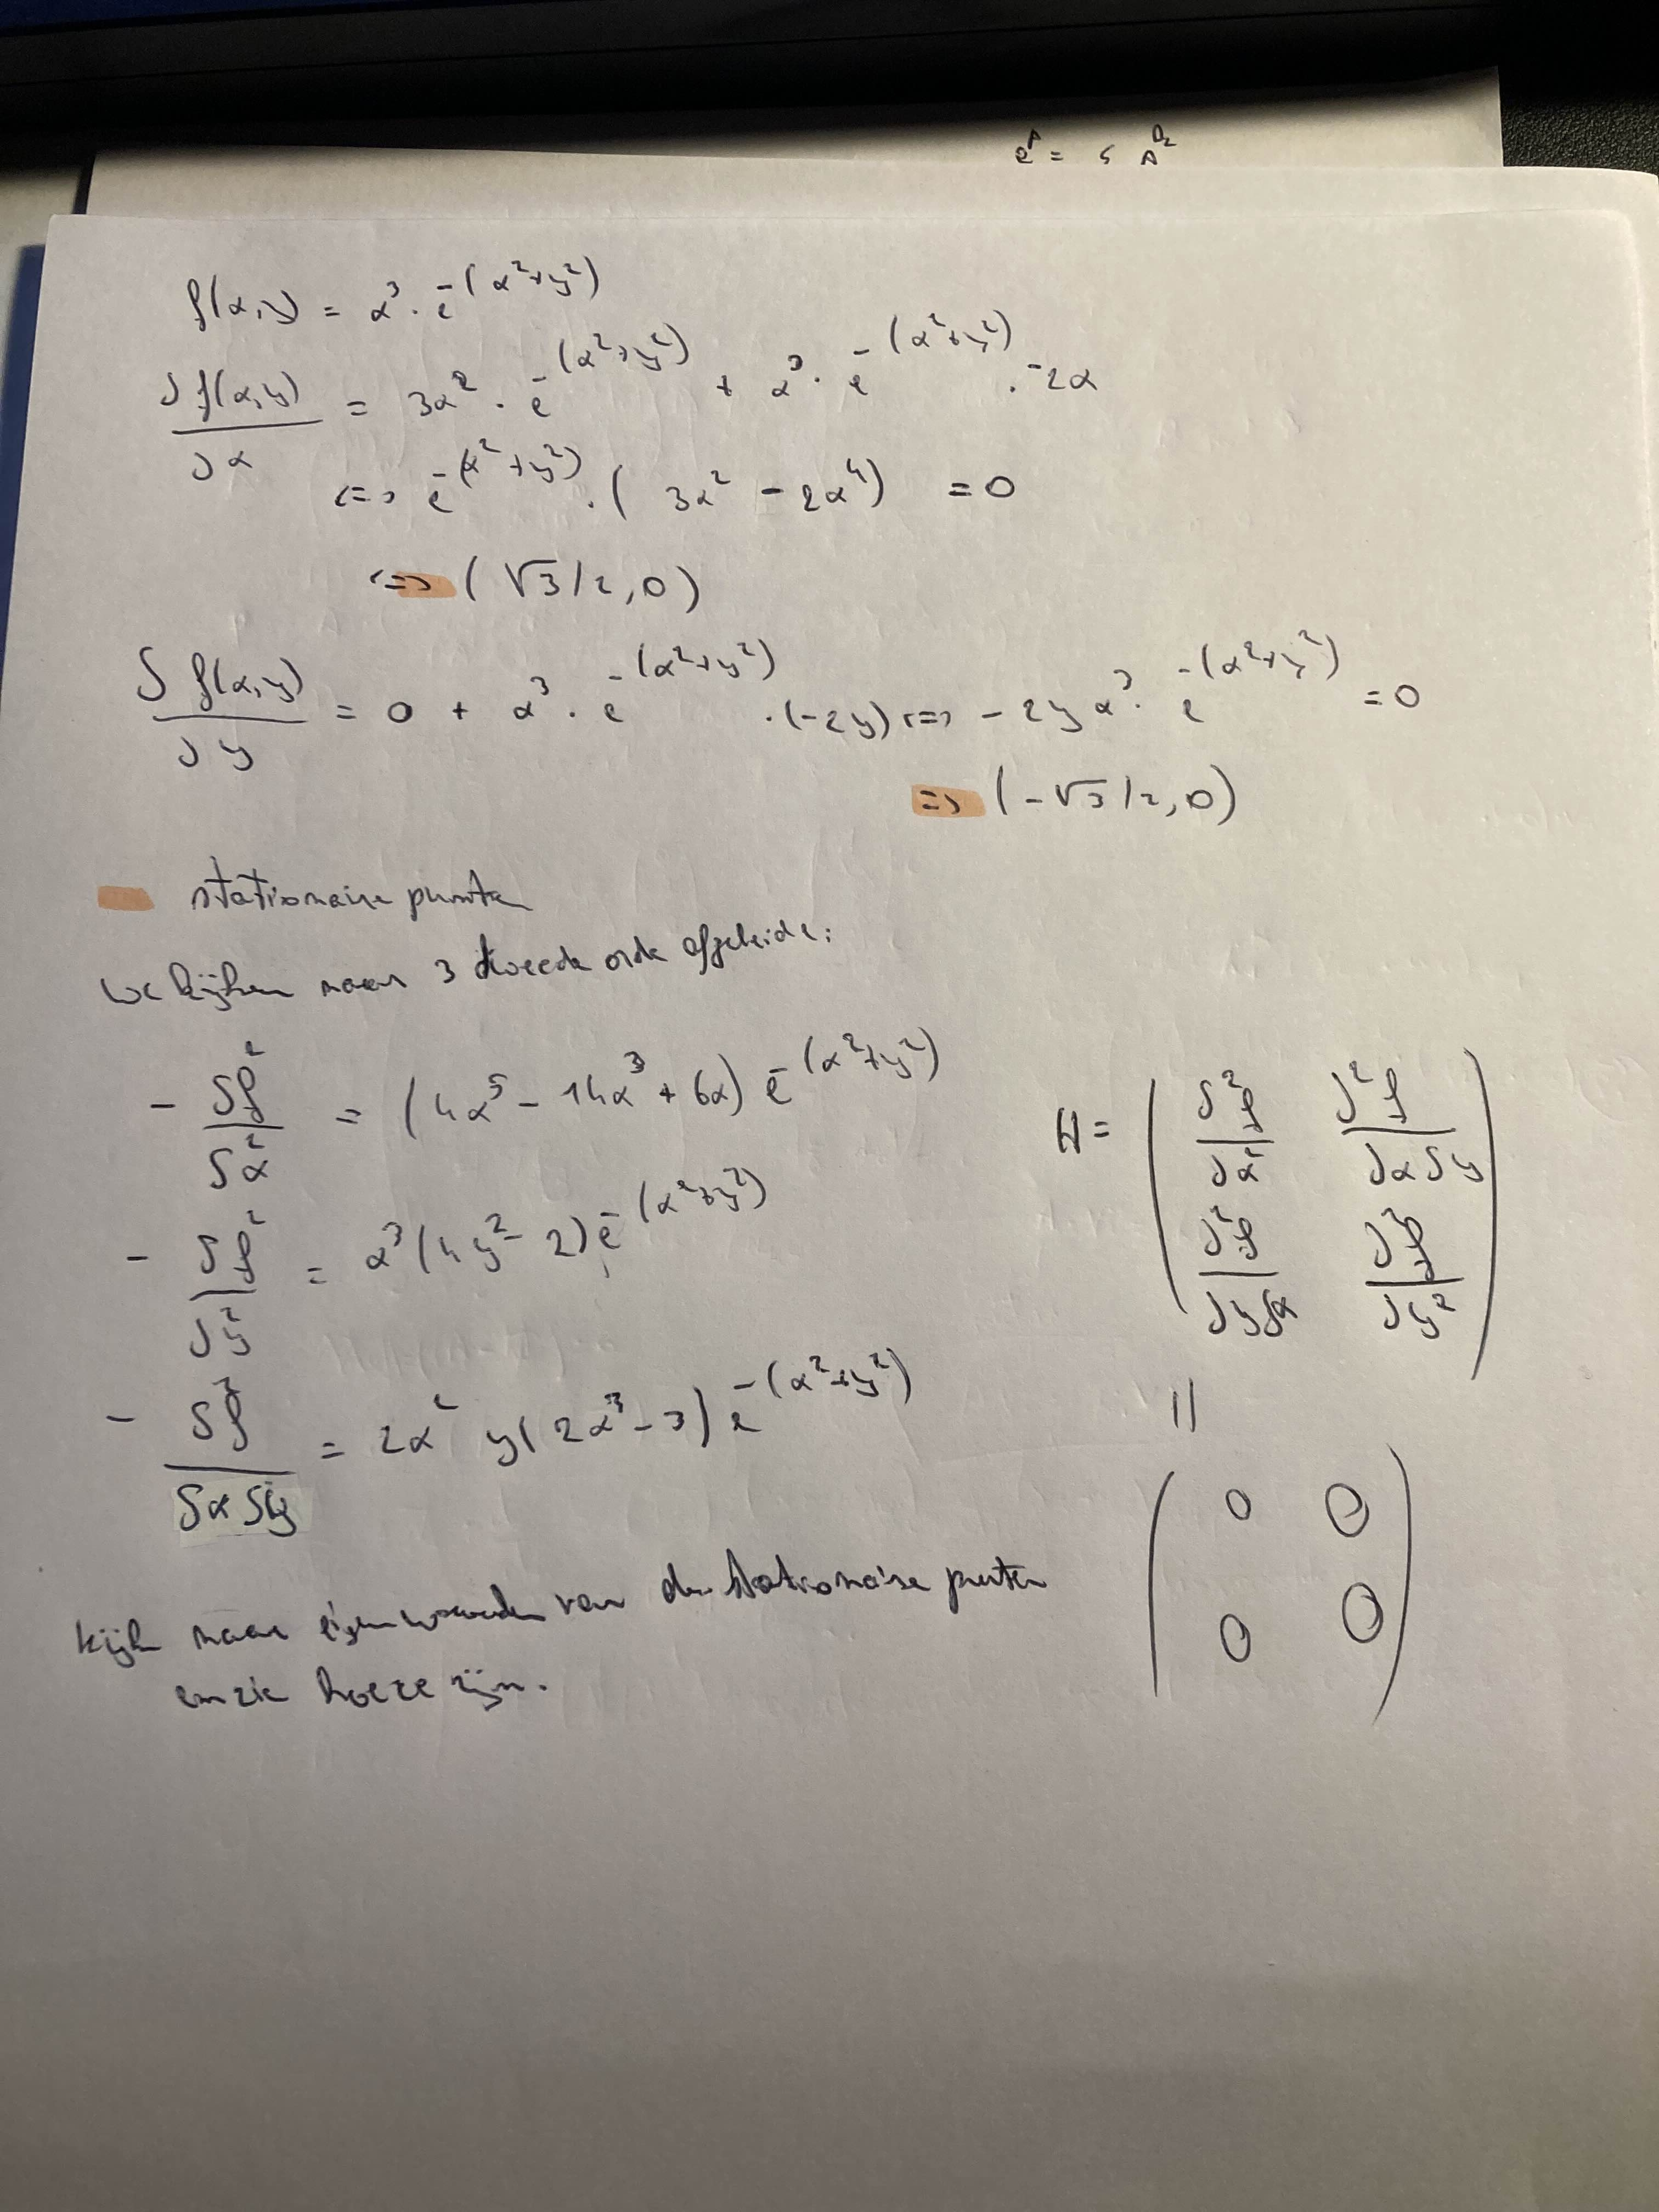
\includegraphics[width=0.95\textwidth]{./images/hessian_my.jpg}
	\end{center}
	\caption{Hessiaan}
	\label{}
\end{figure}

\begin{figure}[H]
	\begin{center}
		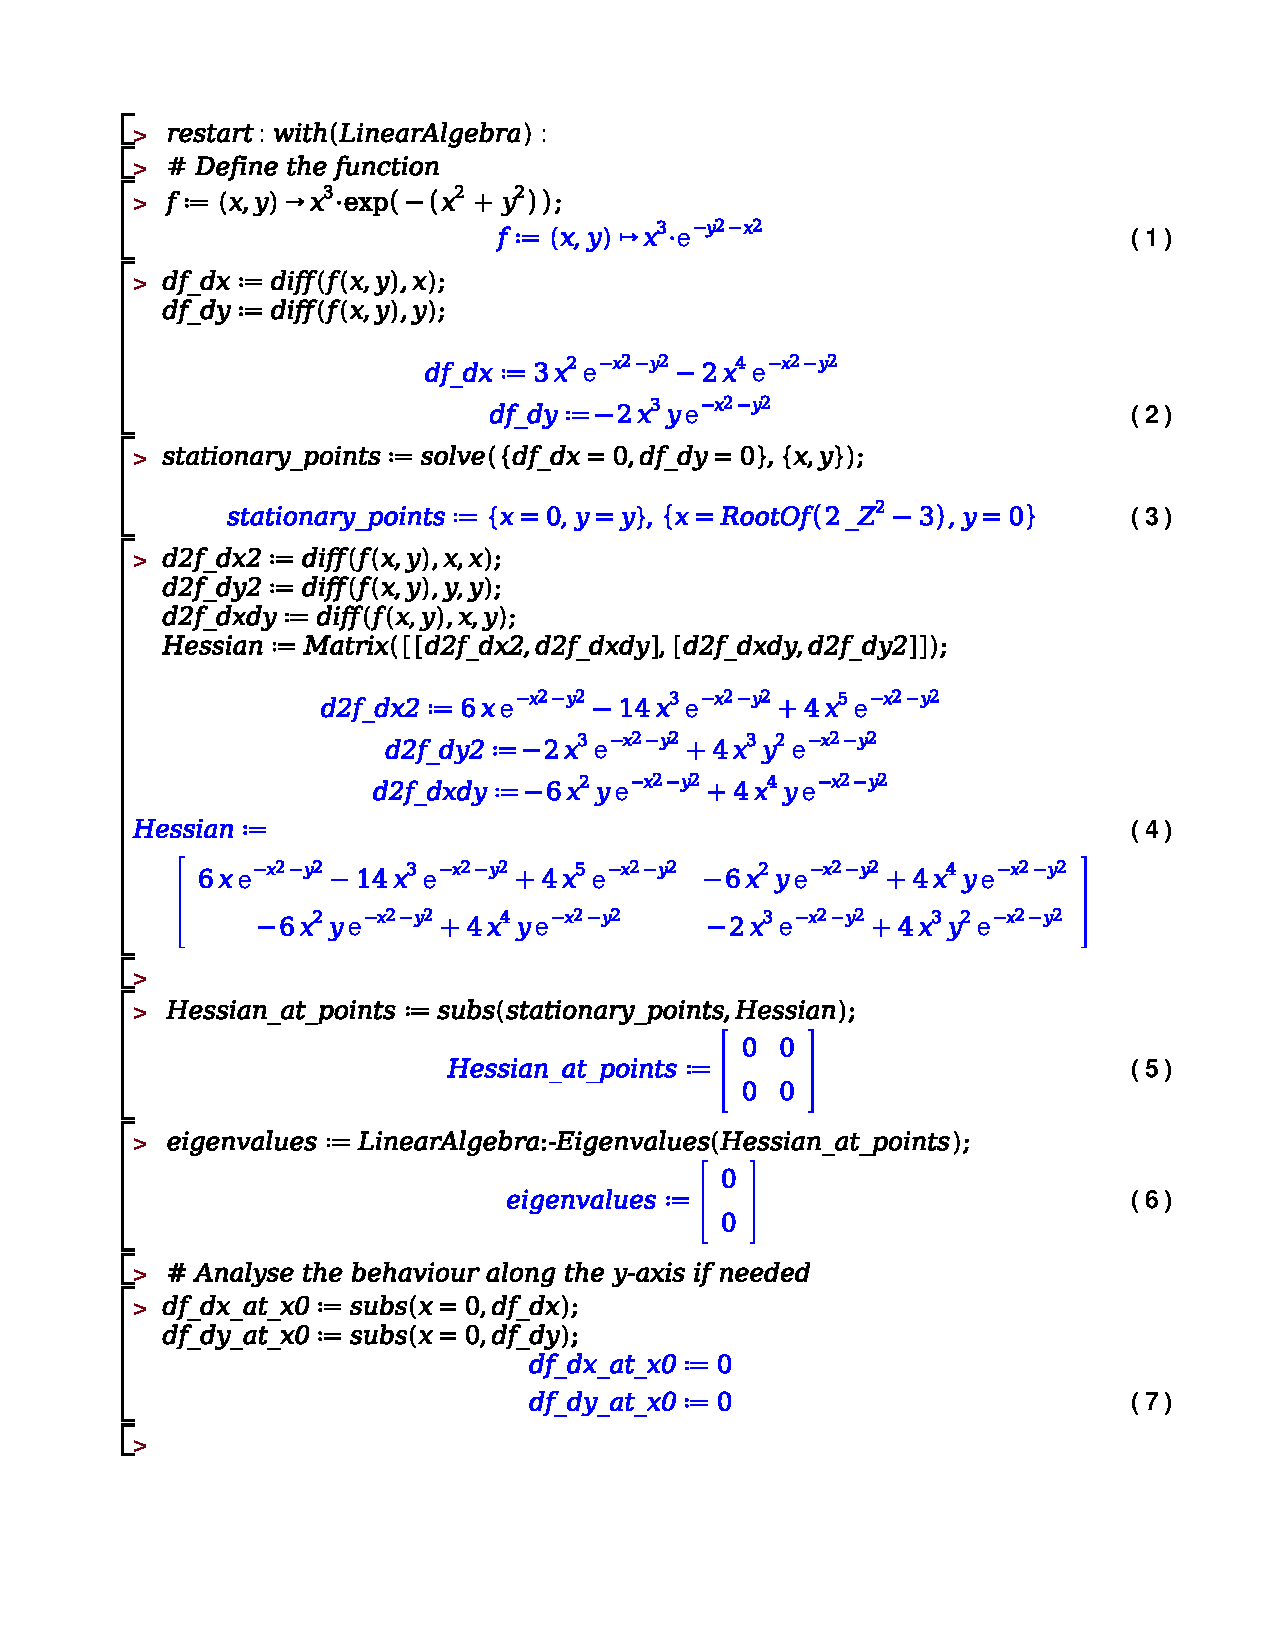
\includegraphics[width=0.95\textwidth]{./hessian.pdf}
	\end{center}
	\caption{Hessiaan}
	\label{}
\end{figure}

\subsection{Integratie}

\subsubsection{De riemanniaanse integraal}

\begin{figure}[H]
	\centering
	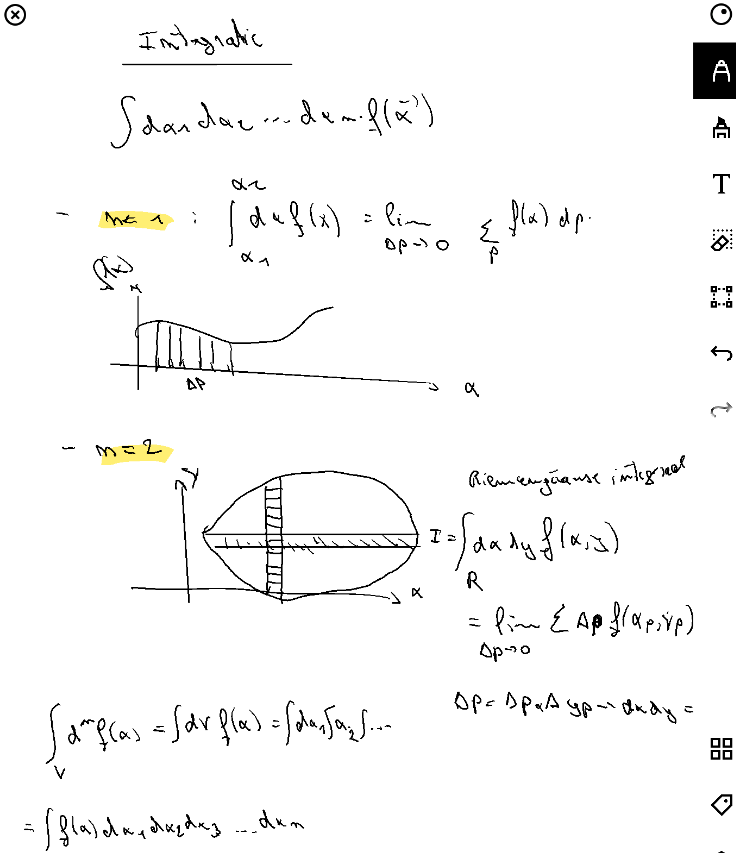
\includegraphics[width=0.8\textwidth]{assets/integralen_uitleg.png}
	\caption{Integratie uitleg}
	\label{fig:integralen_uitleg}
\end{figure}

\subsubsection{Voorbeeld}


\begin{figure}[H]
	\centering
	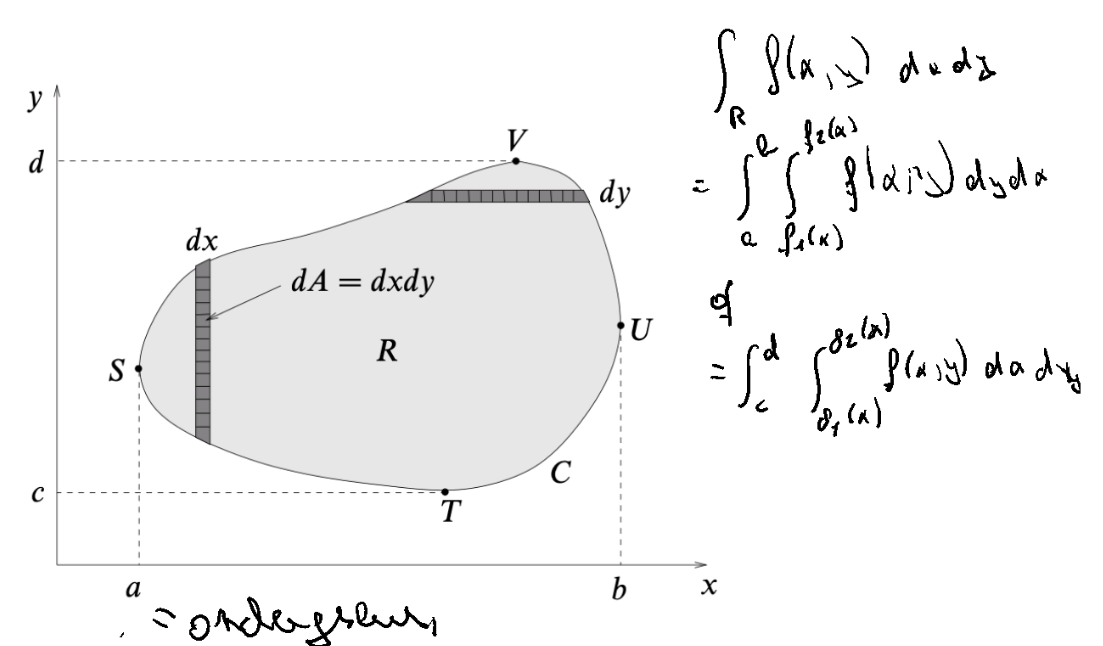
\includegraphics[width=0.8\textwidth]{assets/integraal_oppervalk.png}
	\caption{Integraal oppervlak}
	\label{fig:integraal_oppervalk}
\end{figure}


\subsubsection{Voorbeeld}


\begin{figure}[H]
	\centering
	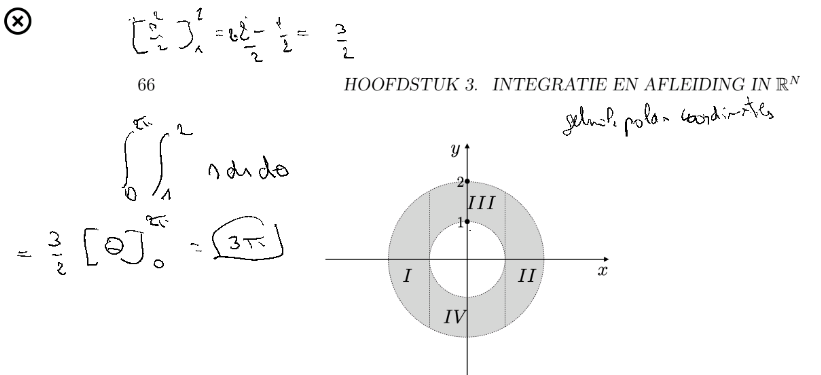
\includegraphics[width=0.8\textwidth]{assets/circkel_oppervlak.png}
	\caption{Cirkel oppervlak}
	\label{fig:circkel_oppervlak}
\end{figure}

Dit kan ook via de (x, y) coordinaten, waarbij de cirkel wordt voorgesteld door: $x^2 + y^2 = r^2$, dan krijg je:


\begin{figure}[H]
	\centering
	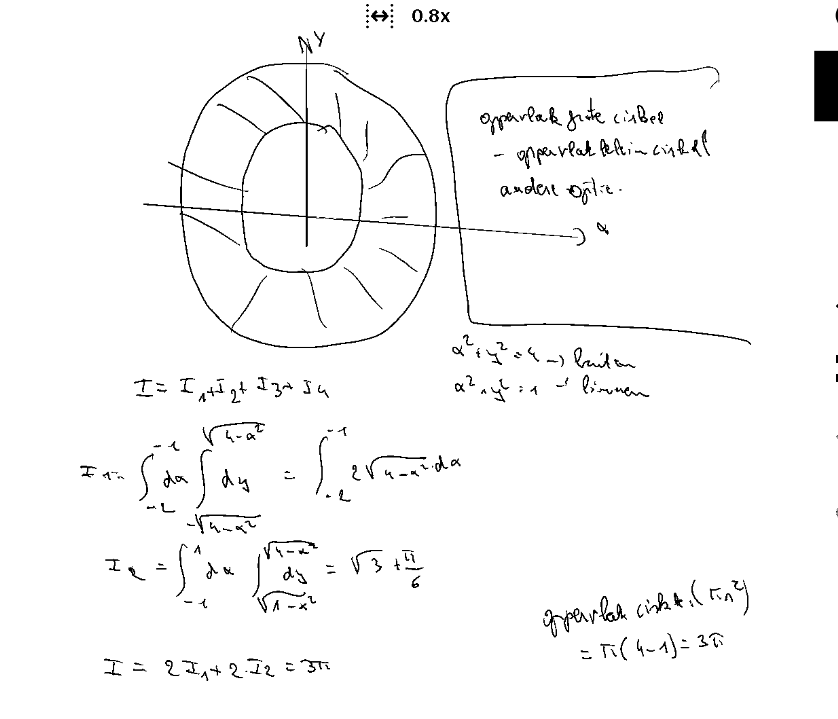
\includegraphics[width=0.8\textwidth]{assets/oppervlak_cirkel_x_y.png}
	\caption{Oppervlak cirkel x, y}
	\label{fig:oppervlak_cirkel_x_y}
\end{figure}

We kunnen ook volumes bereken, is basically een triple integraal...

\subsubsection{Voorbeeld}


\begin{figure}[H]
	\centering
	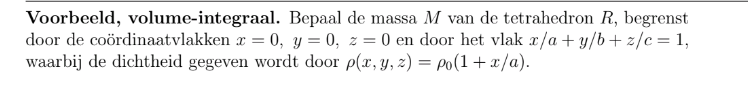
\includegraphics[width=0.8\textwidth]{assets/volume_vraag.png}
	\caption{Volume vraag}
	\label{fig:volume_vraag}
\end{figure}


\begin{figure}[H]
	\centering
	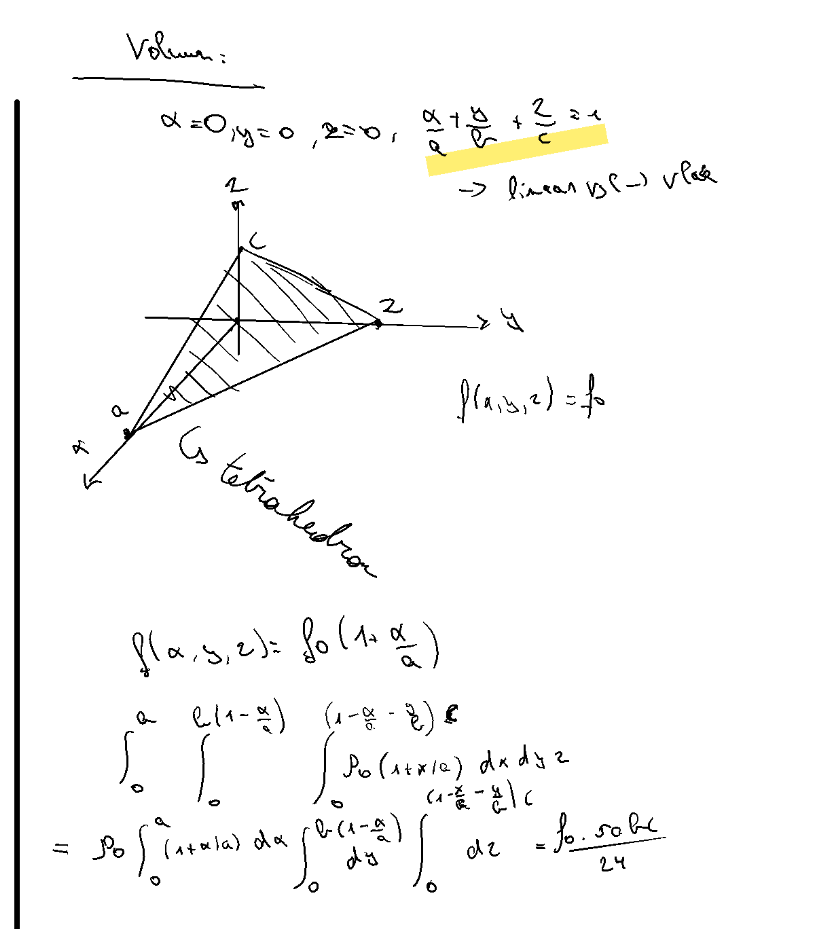
\includegraphics[width=0.8\textwidth]{assets/volume_sol.png}
	\caption{Volume solution}
	\label{fig:volume_sol}
\end{figure}

Een paar typische toepassingen zijn:


\begin{figure}[H]
	\centering
	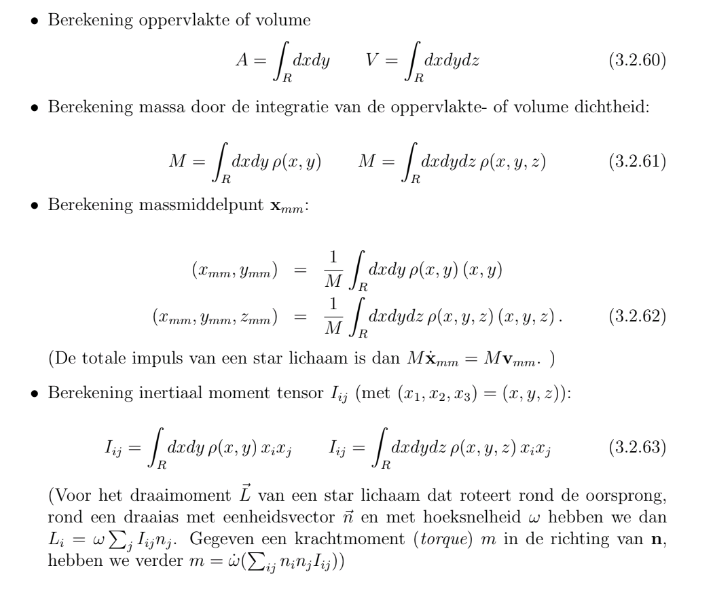
\includegraphics[width=0.8\textwidth]{assets/typische_integralen.png}
	\caption{Typische integralen}
	\label{fig:typische_integralen}
\end{figure}

\subsection{Verandering integratievariabelen}

Basically we willen de integraal veranderen van coordinatenstelsel. Dit kan via de Jacobiaan.


\begin{figure}[H]
	\centering
	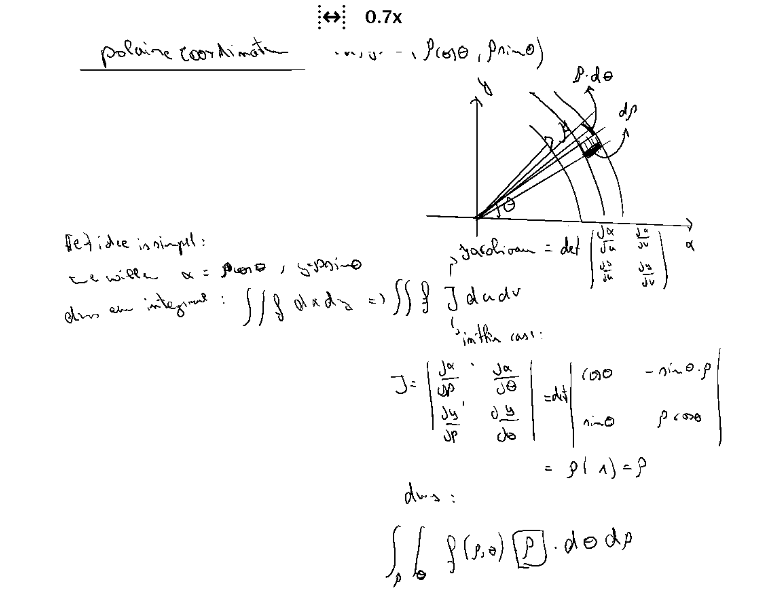
\includegraphics[width=0.8\textwidth]{assets/voorbeeld_coordinaten_transfo_integralen.png}
	\caption{Voorbeeld coordinaten transformatie}
	\label{fig:voorbeeld_coordinaten_transfo_integralen}
\end{figure}


\subsection{Pool-, cilinder- en bolcoordinaten}


\begin{figure}[H]
	\centering
	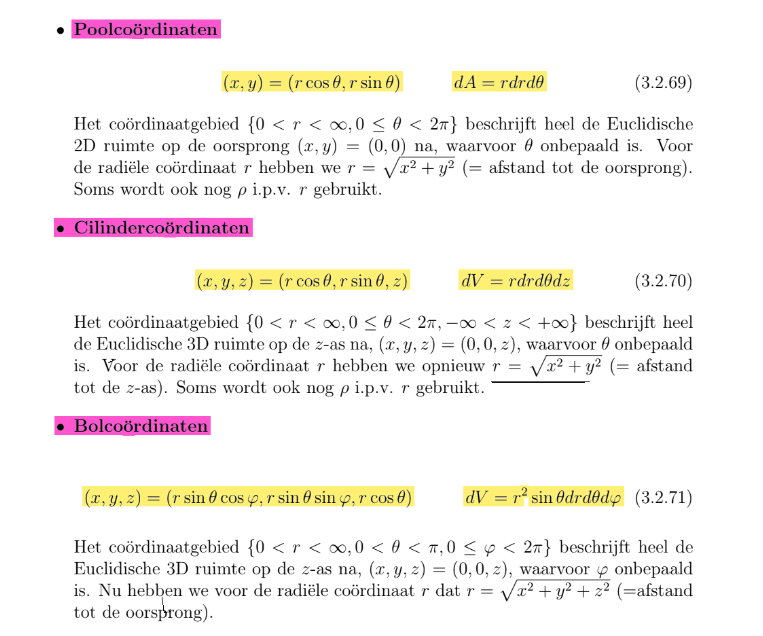
\includegraphics[width=0.8\textwidth]{assets/pool_cilinder_bol_coordinaten.png}
	\caption{Pool, cilinder en bol coordinaten}
	\label{fig:pool_cilinder_bol_coordinaten}
\end{figure}


\subsubsection{Voorbeeld}


\begin{figure}[H]
	\centering
	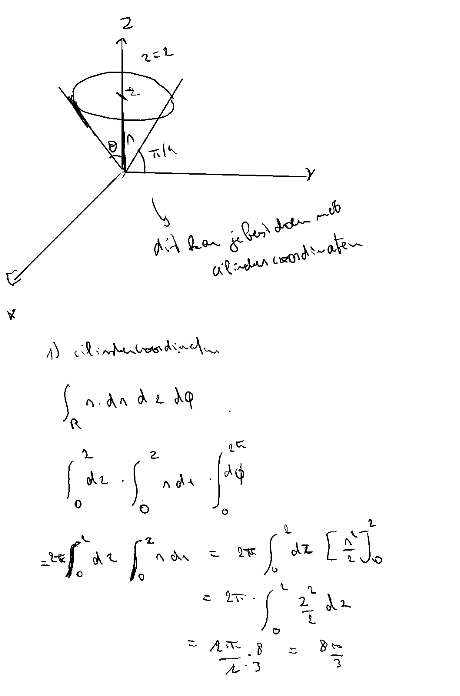
\includegraphics[width=0.8\textwidth]{assets/voorbeeld_pool_coordinaten.png}
	\caption{Voorbeeld pool coordinaten}
	\label{fig:voorbeeld_pool_coordinaten}
\end{figure}

\chapter{Vectoranalyse in drie dimensies }

\subsection{Vectoren en vector bewerkingen}

\subsubsection{Scalair product, norm, afstand}

\begin{figure}[H]
	\centering
	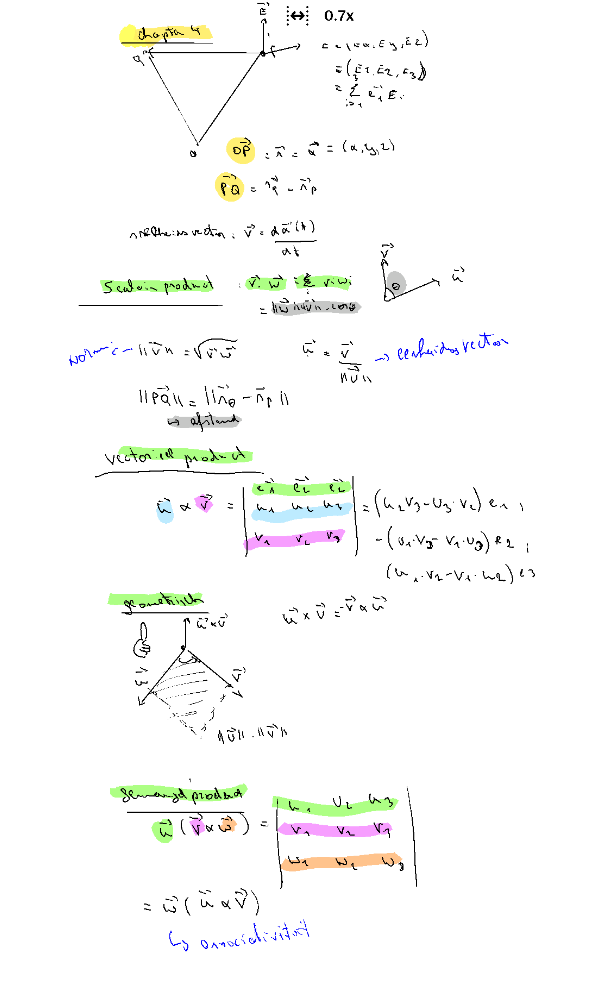
\includegraphics[width=0.8\textwidth]{assets/termen_h4.png}
	\caption{Definities}
	\label{fig:termen_h4}
\end{figure}

Belangrijk om te weten is dat $w = u \times v$ de vector is die loodrecht staat op $u$ en $v$.

\textbf{Triple product}: $u \times (v \times w) =  (u . w) . v - (u . v) . w$

\subsection{Vector velden en vectoriele afleiding}

\subsubsection{Vector- en scalaire velden: Maxwell en Navier-Stokes}

Hier een paar vergelijkingen die je \textbf{niet} moet kennen maar wel moet kunnen bewijzen:


\begin{figure}[H]
	\centering
	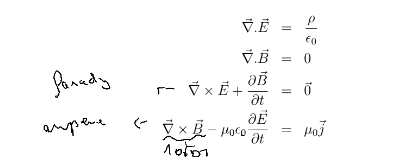
\includegraphics[width=0.8\textwidth]{assets/maxwell.png}
	\caption{Maxwell laws}
	\label{fig:maxwell}
\end{figure}

De navier-stokes vergelijkingen beschrijven gas/liquid flow en zijn als volgt:

\begin{figure}[H]
	\centering
	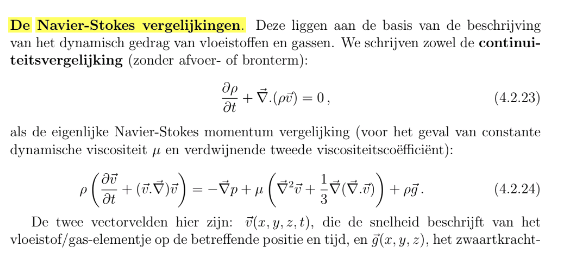
\includegraphics[width=0.8\textwidth]{assets/navier_stokes.png}
	\caption{Navier-Stokes}
	\label{fig:navier_stokes}
\end{figure}

\subsubsection{Conservatieve velden}

\begin{figure}[H]
	\centering
	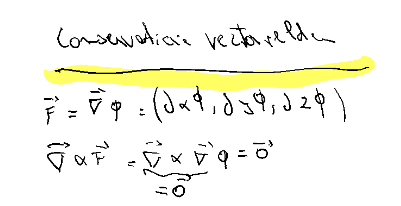
\includegraphics[width=0.8\textwidth]{assets/conservatieve_velden.png}
	\caption{Conservatieve velden}
	\label{fig:conservatieve_velden}
\end{figure}

Een vectorveld wordt conservatief genoemd wanneer deze kan herschreven worden als een gradient van een scalair veld $\phi$

$F = \nabla \phi$

Samengevat: voor een ESG (enkelvoudig samenhangend gebied) is een vectorveld conservatief als de rotor = 0, $\nabla \times F = 0$. Hierbij hebben we dan ook het feit dat het vectorveld conservatief is: $F = \nabla \phi$

\textbf{ESG} btw is een gebied die we kunnen herleiden tot een punt. Dus stel er is een paal midden in het gebied, is dit geen ESG want we de paal staat in de weg!


\begin{figure}[H]
	\centering
	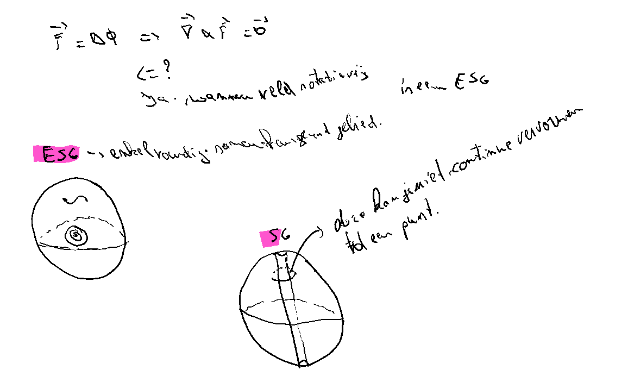
\includegraphics[width=0.8\textwidth]{assets/ESG.png}
	\caption{ESG}
	\label{fig:esg}
\end{figure}

\subsubsection{Voorbeeld}

\begin{figure}[H]
	\centering
	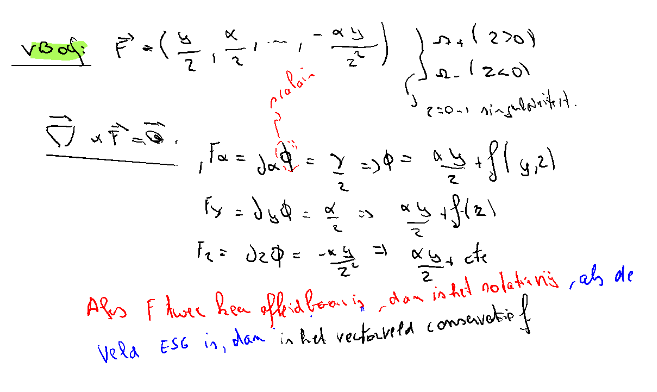
\includegraphics[width=0.8\textwidth]{assets/voorbeeld_rotor_conservatief.png}
	\caption{Voorbeeld rotor conservatief}
	\label{fig:voorbeeld_rotor_conservatief}
\end{figure}


\subsubsection{The Fab Four: gradient, divergentie, laplaciaan, rotor}

\begin{enumerate}

	\item Gradient: $\nabla = (\partial_x, \partial_y, \partial_z)$
	\item Divergentie: Als we de gradient combineren met een vector veld, krijgen we de divergentie. Dit is een scalaire waarde. $\nabla . E = \frac{\partial E_x}{\partial x} + \frac{\partial E_y}{\partial y} + \frac{\partial E_z}{\partial z}$
	\item Laplaciaan: Is letterlijk gewoon gradient maar twee keer partieel afleiden per component... $\nabla . \nabla = \triangle = \frac{\partial^2}{\partial x^2} + \frac{\partial^2}{\partial y^2} + \frac{\partial^2}{\partial z^2}$
\end{enumerate}

// Note: De toepassing in de cursus wordt nooit op die manier gegeven... Skip

Nog iets heel belangrijk: \textbf{Rotor}: $\nabla \times E = \begin{bmatrix} e_1 & e_2 & e_3 \\ \partial_x & \partial_y & \partial_z \\ E_x & E_y & E_z \\ \end{bmatrix}$

Als rotor = 0, dan is het veld conservatief.

\subsection{Nabla calculus}

Dit zijn basically a bunch of formulas die je moet kunnen bewijzen:


\begin{figure}[H]
	\centering
	\includegraphics[width=0.8\textwidth]{assets/bewijzen_nabla_calculus.png}
	\caption{Bewijzen nabla calculus}
	\label{fig:bewijzen_nabla_calculus}
\end{figure}


\begin{figure}[H]
	\centering
	\includegraphics[width=0.8\textwidth]{assets/sommige_bewijzen_nabla_calculus.png}
	\caption{Sommige bewijzen nabla calculus}
	\label{fig:sommige_bewijzen_nabla_calculus}
\end{figure}

\subsubsection{Solenoïdale vector velden}

\textbf{solenoidal} is wanneer we het volgende hebben: $F = \nabla \times A$ (Hierbij is $F$ dus solenoidal)

Met $A$ het \textbf{Vector potentiaal}.

Wanneer we $\nabla . F = 0$ dan is onze solenoidal vectorveld ook \textbf{divergentie vrij}.

Belangrijk volgende relatie: $F = \nabla \times A$ (solenoidal) $\equiv \nabla . F = 0$ (divergentie vrij)

Zoals bij de Conservatie velden, wanneer het veld niet ESG is, kunnen we niet convergeren naar 1 punt en dus $F \neq \nabla \times A$

\subsubsection{Voorbeeld}


\begin{figure}[H]
	\centering
	\includegraphics[width=0.8\textwidth]{assets/sinusoidal_example.png}
	\caption{Sinusoidal example}
	\label{fig:sinusoidal_example}
\end{figure}

It's very easy to see that the field is solenoidal, just take gradient and boem $= (0,0,0)$

Then we find $A$:


\begin{figure}[H]
	\centering
	\includegraphics[width=0.8\textwidth]{assets/solenoide_solution.png}
	\caption{Solenoide solution}
	\label{fig:solenoide_solution}
\end{figure}

\subsubsection{Helmholtz decompositie}

In een ESG kunnen we een vectorveld decomposeren in een solenoidal en een conservatief veld.

$F = \nabla \phi + \nabla \times A$ (eerste term is conservatief, tweede term is solenoidal)

Note: Dit is een \textbf{poissonvergelijking}

Die je kunt berekenen door het volgende te doen:

$\pi(x) = - \int \frac{\rho(x')}{||x - x'|| . 4\pi} d^3 x'$

\subsubsection{Voorbeeld}


\begin{figure}[H]
	\centering
	\includegraphics[width=0.8\textwidth]{assets/helmholtz_example.png}
	\caption{Helmholtz example}
	\label{fig:helmholtz_example}
\end{figure}

\begin{figure}[H]
	\centering
	\includegraphics[width=0.8\textwidth]{assets/helmholtz_maple.png}
	\caption{Helmholtz maple}
	\label{fig:helmholtz_maple}
\end{figure}

\begin{figure}[H]
	\centering
	\includegraphics[width=0.8\textwidth]{assets/helmholtz_sol.png}
	\caption{Helmholtz solution}
	\label{fig:helmholtz_sol}
\end{figure}

\subsection{Integratie}

\subsubsection{Lijnintegralen}

Is een integraal over een kromme $C$ waarbij de lijnintegraal niet afhangt van de zin waarmee de kromme wordt doorlopen.

\textbf{[A] Booglengte, dichtheid, massamiddelpunt, ...}:

Stel we willen een koord lengte definieren, dit kunnen we doen door:

$ds = \sqrt{dx . dx}$

met $dx = \frac{dx}{dt} dt$

waarbij $\frac{dx}{dt}$ de \textbf{raakvector} is.

Hierbij mijn notities over het concept:


\begin{figure}[H]
	\centering
	\includegraphics[width=0.8\textwidth]{assets/notities_lijn_integraal.png}
	\caption{Notities lijn integraal}
	\label{fig:notities_lijn_integraal}
\end{figure}

\subsubsection{Voorbeeld}

\begin{figure}[H]
	\centering
	\includegraphics[width=0.8\textwidth]{assets/voorbeeld_lijn_integraal.png}
	\caption{Voorbeeld lijn integraal}
	\label{fig:voorbeeld_lijn_integraal}
\end{figure}


\begin{figure}[H]
	\centering
	\includegraphics[width=0.8\textwidth]{assets/lijnintegraal_solution.png}
	\caption{Lijnintegraal solution}
	\label{fig:lijnintegraal_solution}
\end{figure}


\begin{figure}[H]
	\centering
	\includegraphics[width=0.8\textwidth]{assets/example_lijnintegraal_massa_middelpunt.png}
	\caption{Example lijnintegraal massa middelpunt}
	\label{fig:example_lijnintegraal_massa_middelpunt}
\end{figure}


\textbf{[B] Vectorvelden: $\int F.dx$, $\int F \times dx$}:

Hier hetzelfde als bij punt [A], maar nu definieren we de volgende integraal:


\begin{figure}[H]
	\centering
	\includegraphics[width=0.8\textwidth]{assets/integraal_vectorvelden.png}
	\caption{}
	\label{fig:integraal_vectorvelden}
\end{figure}

nog een ander type integraal is de volgende:


\begin{figure}[H]
	\centering
	\includegraphics[width=0.8\textwidth]{assets/integraal_vector_velden_cross_product.png}
	\caption{Ingtegraal vector velden type 2}
	\label{fig:integraal_vector_velden_cross_product}
\end{figure}

\subsubsection{Voorbeeld}

\begin{figure}[H]
	\centering
	\includegraphics[width=0.8\textwidth]{assets/voorbeeld_lijn_integraal_vectorveld.png}
	\caption{Voorbeeld lijn integraal vectorveld}
	\label{fig:voorbeeld_lijn_integraal_vectorveld}
\end{figure}


\subsubsection{Voorbeeld}

\begin{figure}[H]
	\centering
	\includegraphics[width=0.8\textwidth]{assets/voorbeeld_tornado.png}
	\caption{Voorbeeld tornado}
	\label{fig:voorbeeld_tornado}
\end{figure}

\subsubsection{Voorbeeld}

\begin{figure}[H]
	\centering
	\includegraphics[width=0.8\textwidth]{assets/biost_savant.png}
	\caption{}
	\label{fig:biost_savant}
\end{figure}

\subsection{Oppervlakeintegralen}


\begin{figure}[H]
	\centering
	\includegraphics[width=0.8\textwidth]{assets/oppervlakte_integraal_uitleg.png}
	\caption{Oppervlakte integralen: maw, we gaan de oppervlakte in 3D berekenen door $\int \int du dv norm(du \times dv)$}
	\label{fig:oppervlakte_integraal_uitleg}
\end{figure}

\subsubsection{Voorbeeld}

\begin{figure}[H]
	\centering
	\includegraphics[width=0.8\textwidth]{assets/voorbeeld_boloppervlak.png}
	\caption{Voorbeeld boloppervlak}
	\label{fig:voorbeeld_boloppervlak}
\end{figure}

\begin{figure}[H]
	\centering
	\includegraphics[width=0.8\textwidth]{assets/voorbeeld_boloppervlak_oplossing.png}
	\caption{Voorbeeld boloppervlak oplossing}
	\label{fig:voorbeeld_boloppervlak_oplossing}
\end{figure}

\begin{figure}[H]
	\centering
	\includegraphics[width=0.8\textwidth]{assets/cilinder_oppervlak_oplossing.png}
	\caption{Cilinder oppervlak oplossing}
	\label{fig:cilinder_oppervlak_oplossing}
\end{figure}

Dan is er ook een toepassing van flux doorheen een oppervlak die kan uitgelegd worden met de volgende afbeelding:


\begin{figure}[H]
	\centering
	\includegraphics[width=0.8\textwidth]{assets/flux_voorbeeld.png}
	\caption{Flux voorbeeld}
	\label{fig:flux_voorbeeld}
\end{figure}

\subsection{Integratiestellingen}

\begin{figure}[H]
	\centering
	\includegraphics[width=0.8\textwidth]{assets/IntegratieStellingen.png}
	\caption{Integratie stellingen}
	\label{fig:integratiestellingen}
\end{figure}


Hier zien we \textbf{Stokes}, \textbf{divergentiestelling van Gauss}, en \textbf{Stelling van Green}. \textbf{Stokes} is een generalizatie van \textbf{Green}. Het idee van stokes is dat we een 2D integraal die de oppervlakte integraal is van een rotor \textbf{herleidt} tot een lijnintegraal over de rand.

\begin{figure}[H]
	\centering
	\includegraphics[width=0.8\textwidth]{assets/Stelling van Stokes.png}
	\caption{Stelling van Stokes}
	\label{fig:stelling-van-stokes}
\end{figure}

Nu we weten wat Stokes eigenlijk is, laten we een voorbeeld bezichtigen:


\begin{figure}[H]
	\centering
	\includegraphics[width=0.8\textwidth]{assets/stokes_voorbeeld_opgelost.png}
	\caption{Stokes voorbeeld opgelost}
	\label{fig:stokes_voorbeeld_opgelost}
\end{figure}


\begin{figure}[H]
	\centering
	\includegraphics[width=0.8\textwidth]{assets/uitleg_green.png}
	\caption{Uitleg Green}
	\label{fig:uitleg_green}
\end{figure}


Aan de andere kant heb je de divergentiestelling, waarbij we een 3D volume integraal van de divergentie tot een oppervlak integraal over de randoppervlak kunnen herleiden.

\begin{figure}[H]
	\centering
	\includegraphics[width=0.8\textwidth]{assets/divergentie_stelling.png}
	\caption{Divergentie stelling}
	\label{fig:divergentie_stelling}
\end{figure}

Of gewoon in formule:

\begin{figure}[H]
	\centering
	\includegraphics[width=0.8\textwidth]{assets/formule_divergentie_wet.png}
	\caption{Formule Divergentiestelling}
	\label{fig:formule_divergentie_wet}
\end{figure}

Als je dan de stelling van Gauss wilt bekijken wordt het als volgt gedaan:

\begin{figure}[H]
	\centering
	\includegraphics[width=0.8\textwidth]{assets/voorbeeld_gauss_toepassing.png}
	\caption{Voorbeeld Gauss toepassing}
	\label{fig:voorbeeld_gauss_toepassing}
\end{figure}

Zoals de prof het zei: "Ik ben trots op deze figuur". Hier gaan we zien dat de 2 inifitismale oppervlaktes een shared boundary hebben, deze worden te niet gezien, waardoor je uiteindelijk 1 lijn integraal krijgt over die twee vlakjes, extrapoleer nu naar de rest en zo bewijs je dus dat \textbf{Stokes} een Top G is.
Btw, de rechterhand regel leert ons dan welke teken de lijnintegraal nodig heeft.

\begin{figure}[H]
	\centering
	\includegraphics[width=0.8\textwidth]{assets/inzicht_integraalstellingen.png}
	\caption{Inzicht integratie stellingen}
	\label{fig:inzicht_integraalstellingen}
\end{figure}

\subsection{Toepassing: Continuiteitsvergelijking}

Het komt erop neer dat dit fysische toepassingen zijn waarbij we de wet van behoud van massa toepassen. Dit is een toepassing van de divergentiestelling. (een voorbeeld)

Het ander voorbeeld is behoudt van lading:

\begin{figure}[H]
	\centering
	\includegraphics[width=0.8\textwidth]{assets/lading.png}
	\caption{Lading}
	\label{fig:lading}
\end{figure}

\chapter{Gewone Lineaire Differentiaalvergelijkingen}

Note: Dit is meer een oefening gerichte hoofdstuk.

Eerst definieren we een paar termen:

\begin{figure}[H]
	\centering
	\includegraphics[width=0.8\textwidth]{assets/termen_hf5.png}
	\caption{Termen}
	\label{fig:termen_hf5}
\end{figure}

In woorden: Homogeen heeft geen source, linear wel, orde wordt bepaald door de hoogste afgeleide, en differentiaalvergelijkingen zijn gewoon vergelijkingen met afgeleiden.

\subsection{Voorbeelden}

\begin{figure}[H]
	\centering
	\includegraphics[width=0.8\textwidth]{assets/some_DV_examples.png}
	\caption{Some DV examples}
	\label{fig:some_dv_examples}
\end{figure}

\textbf{Wronkiaan}: Dit is een determinant van de matrix van de afgeleiden van de functies. Als deze determinant = 0, dan zijn de functies lineair afhankelijk.
We willen meestal checkecn of een matrix lineair onafhankelijk is, dit doen we door de determinant te berekenen en zien of het $\neq 0$.

$$ W = \begin{vmatrix} y_1 & y_2 & y_3 \\ y_1' & y_2' & y_3' \\ y_1'' & y_2'' & y_3'' \end{vmatrix} $$

\begin{figure}[H]
	\centering
	\includegraphics[width=0.8\textwidth]{assets/wronskiaan_voorbeeld.png}
	\caption{Wronskiaan voorbeeld}
	\label{fig:wronskiaan_voorbeeld}
\end{figure}

Hoe bepalen we de verschillende oplossingen van een differentiaalvergelijking?


\begin{figure}[H]
	\centering
	\includegraphics[width=0.8\textwidth]{assets/bepalen_y_i.png}
	\caption{Bepalen $y_i$}
	\label{fig:bepalen_y_i}
\end{figure}


\begin{figure}[H]
	\centering
	\includegraphics[width=0.8\textwidth]{assets/voorbeeld_dv_calc.png}
	\caption{Voorbeeld DV calc}
	\label{fig:voorbeeld_dv_calc}
\end{figure}

Dan heb je ook het concept van particuliere oplossingen, dit zijn oplossingen die je zelf moet vinden. Dit kan je doen door de methode van de variatie van de constanten toe te passen.
Aka, je neemt de algemene oplossing en je gaat de constanten veranderen naar functies.

\begin{figure}[H]
	\centering
	\includegraphics[width=0.8\textwidth]{assets/particuliere_oplossingen.png}
	\caption{Particuliere oplossingen}
	\label{fig:particuliere_oplossingen}
\end{figure}

\subsection{Beginvoorwaarden calculeren}

Essentially, we gaan de beginvoorwaarden gebruiken om de constanten te berekenen. Dit doen we door de functie in te vullen in de differentiaalvergelijking en dan de constanten te berekenen.

\begin{figure}[H]
	\centering
	\includegraphics[width=0.8\textwidth]{assets/beginvoorwaarden_calculatie.png}
	\caption{Beginvoorwaarden calculatie}
	\label{fig:beginvoorwaarden_calculatie}
\end{figure}

\subsection{Rand versus beginvoorwaarden probleem}

\begin{figure}[H]
	\centering
	\includegraphics[width=0.8\textwidth]{assets/rand-vs-beginvoorwaarden.png}
	\caption{Rand vs beginvoorwaarden}
	\label{fig:rand-vs-beginvoorwaarden}
\end{figure}

De professor vond het ook leuk om een beetje fysica toe te voegen:

\begin{figure}[H]
	\centering
	\includegraphics[width=0.8\textwidth]{assets/rlc-stuff.png}
	\caption{RLC en gedempte trillingen}
	\label{fig:rlc-stuff}
\end{figure}

\section*{Formularium}

\subsection*{Taylorontwikkeling}

- $ f(x) = f(a) + f'(a)(x-a) + \frac{f''(a)}{2!}(x-a)^2 + \frac{f'''(a)}{3!}(x-a)^3 + ... $

- $sin(x) = x$ voor kleine $x$

\subsection*{Differentiaalvergelijkingen}

- $y'(x) = \lambda y(x)$

- $y''(x) = \lambda y(x)$ (hier werden 3 gevallen besproken)

\subsection*{Complexe getallen}

- $z = a + bi$ (algemene vorm)

- $i^2 = -1$

- \textbf{inverse}: $(a + bi)^{-1} = \frac{a - bi}{a^2 + b^2}$

- \textbf{complement}: $z = a + bi \rightarrow z^* = a - bi$

- \textbf{modulus}: $|z| = \sqrt{a^2 + b^2}$

- $e^{i\theta} = cos(\theta) + i sin(\theta)$

- $sin^2(x) + cos^2(x) = 1$

- $sin(x) = \frac{e^{ix} - e^{-ix}}{2i}$

- $sin(2x) = 2sin(x)cos(x)$

- $cos(x) = \frac{e^{ix} + e^{-ix}}{2}$

- $cos(2x) = cos^2(x) - sin^2(x)$

\subsection*{Hoofdstelling van de algebra}

$x_1 = \frac{-b + \sqrt{b^2 - 4ac}}{2a}$

$x_2 = \frac{-b - \sqrt{b^2 - 4ac}}{2a}$

met $b = -4*a*c$

\subsection*{Lineare Algebra}

$\frac{u\dot v}{||u|| ||v||} = cos(\theta)$ // Hoek tussen twee vectoren

$v^{||} = (u_1 \dot y) u_1 + (u_2 \dot y) u_2 + ...$ // Projectie van $v$

\subsection*{Matrixen}

- Jacobiaan: $J = \begin{bmatrix} \frac{\partial x}{\partial u} & \frac{\partial x}{\partial v} \\ \frac{\partial y}{\partial u} & \frac{\partial y}{\partial v} \end{bmatrix}$

\section*{Oefeningen}

\subsection*{Huis 1}

\begin{figure}[!htbp]
	\centering
	\includegraphics[width=0.8\textwidth]{./exercises/huis_1_ex_1.pdf}
	\caption{Exercise 1}
\end{figure}

\begin{figure}[!htbp]
	\centering
	\includegraphics[width=0.8\textwidth]{./exercises/huis_1_ex_2.pdf}
	\caption{Exercise 2}
\end{figure}



\begin{figure}[!htbp]
	\centering
	\includegraphics[width=0.8\textwidth]{assets/huis_1_ex_3.png}
	\caption{Exercise 3}
	\label{fig:huis_1_ex_3}
\end{figure}


\begin{figure}[!htbp]
	\centering
	\includegraphics[width=0.6\textwidth]{assets/huis_1_ex_4.png}
	\caption{Exercise 4}
	\label{fig:huis_1_ex_4}
\end{figure}

\newpage

\subsection*{WC 1}

\begin{figure}[!htbp]
	\centering
	\includegraphics[width=0.8\textwidth]{./exercises/wc_1_ex_1.pdf}
	\caption{Exercise 1}
\end{figure}

\begin{figure}[!htbp]
	\centering
	\includegraphics[width=0.8\textwidth]{./exercises/wc_1_ex_2.pdf}
	\caption{Exercise 2}
\end{figure}

\begin{figure}[!htbp]
	\centering
	\includegraphics[width=0.8\textwidth]{images/wc1_a3.png}
	\caption{Exercise 3}
\end{figure}

\begin{figure}[!htbp]
	\centering
	\includegraphics[width=0.8\textwidth]{./exercises/wc_1_ex_3.pdf}
	\caption{Exercise 3}
\end{figure}

\newpage
\subsection*{Bord 1}

\begin{figure}[!htbp]
	\centering
	\includegraphics[width=0.8\textwidth]{./exercises/bordles_1.pdf}
	\caption{Exercise 1}
\end{figure}

\begin{figure}[!htbp]
	\centering
	\includegraphics[width=0.8\textwidth]{images/ex_2_a.png}
	\caption{Exercise 2}
\end{figure}

\begin{figure}[!htbp]
	\centering
	\includegraphics[width=0.8\textwidth]{./exercises/bordles_1_ex_2.pdf}
	\caption{Exercise 2 part 2 Maple}
\end{figure}

\begin{figure}[!htbp]
	\centering
	\includegraphics[width=\textwidth]{images/pl_1_answer_3.png}
	\caption{Exercise 3}
\end{figure}

\begin{figure}[!htbp]
	\centering
	\includegraphics[width=\textwidth]{images/plot_2.png}
	\caption{Exercise 3 - plot }
\end{figure}

\begin{figure}[!htbp]
	\centering
	\includegraphics[width=\textwidth]{./exercises/bordles_1_ex_3.pdf}
	\caption{Exercise 3}
\end{figure}

\newpage

\subsection*{Huis 2}

\begin{figure}[!htbp]
	\centering
	\includegraphics[width=0.8\textwidth]{assets/huis_2_ex_1.png}
	\caption{Huis 2 Exercise 1}
	\label{fig:huis_2_ex_1}
\end{figure}


\begin{figure}[!htbp]
	\centering
	\includegraphics[width=0.8\textwidth]{assets/huis_2_ex_2.png}
	\caption{Huis 2 Exercise 2}
	\label{fig:huis_2_ex_2}
\end{figure}


\begin{figure}[!htbp]
	\centering
	\includegraphics[width=0.8\textwidth]{assets/huis_2_ex_3.png}
	\caption{Huis 2 Exercise 3}
	\label{fig:huis_2_ex_3}
\end{figure}

\begin{figure}[!htbp]
	\centering
	\includegraphics[width=0.8\textwidth]{images/huis_2_4.png}
	\caption{Huis 2 Exercise 4}
	\label{fig:huis_2_ex_4}
\end{figure}

\begin{figure}[!htbp]
	\centering
	\includegraphics[width=\textwidth]{images/huis_2_maple_4.png}
	\caption{Huis 2 Exercise 4 Maple}
	\label{fig:huis_2_ex_4_maple}
\end{figure}

\begin{figure}[!htbp]
	\centering
	\includegraphics[width=\textwidth]{exercises/huis_2_ex_5.pdf}
	\caption{Huis 2 Exercise 5: We zien dat de projector op het YZ vlak projecteert.}
	\label{fig:huis_2_ex_5}
\end{figure}

\begin{figure}[!htbp]
	\centering
	\includegraphics[width=\textwidth]{images/huis_2_6.png}
	\caption{Huis 2 Exercise 6: Uit de cursus weten we dat er geen basis kan gevonden worden voor $K(A^T)$ en $N(A)$}
	\label{fig:huis_2_ex_6}
\end{figure}

\begin{figure}[!htbp]
	\centering
	\includegraphics[width=\textwidth]{images/huis_2_7.png}
	\caption{Huis 2 Exercise 7}
	\label{fig:huis_2_ex_7}
\end{figure}

\begin{figure}[!htbp]
	\centering
	\includegraphics[width=\textwidth]{exercises/huis_2_ex_7.pdf}
	\caption{Huis 2 Exercise 7 Maple}
	\label{fig:huis_2_ex_7_maple}
\end{figure}

\begin{figure}[!htbp]
	\centering
	\includegraphics[width=\textwidth]{images/huis_2_8.png}
	\caption{Huis 2 Exercise 8}
	\label{fig:huis_2_ex_8}
\end{figure}

\begin{figure}[!htbp]
	\centering
	\includegraphics[width=\textwidth]{assets/huis_2_ex_8.png}
	\caption{Huis 2 Exercise 8 second version}
	\label{fig:huis_2_ex_8_second}
\end{figure}

\begin{figure}[!htbp]
	\centering
	\includegraphics[width=\textwidth]{images/huis_2_9.png}
	\caption{Huis 2 Exercise 9}
	\label{fig:huis_2_ex_9}
\end{figure}

\begin{figure}[!htbp]
	\centering
	\includegraphics[width=\textwidth]{exercises/huis_2_ex_9.pdf}
	\caption{Huis 2 Exercise 9 Maple}
	\label{fig:huis_2_ex_9_maple}
\end{figure}

\subsection*{Bord 2}


\begin{figure}[!htbp]
	\centering
	\includegraphics[width=\textwidth]{assets/bordles_2_ex_1.png}
	\caption{Bord 2 Exercise 1}
	\label{fig:bord_2_ex_1}
\end{figure}

\begin{figure}[!htbp]
	\centering
	\includegraphics[width=\textwidth]{exercises/bordles_2_ex_1_version_1.pdf}
	\caption{Bord 2 Exercise 1 Maple}
	\label{fig:bord_2_ex_1_maple}
\end{figure}
\begin{figure}[!htbp]
	\centering
	\includegraphics[width=\textwidth]{exercises/bordles_2_ex_1_version_2.pdf}
	\caption{Bord 2 Exercise 1 Maple Version 2: Warning, pdf is not fully loaded, go look in my files}
	\label{fig:bord_2_ex_1_maple_2}
\end{figure}

\begin{figure}[!htbp]
	\centering
	\includegraphics[width=\textwidth]{assets/bordles_2_ex_2.png}
	\caption{Bord 2 Exercise 2}
	\label{fig:bord_2_ex_2}
\end{figure}

\begin{figure}[!htbp]
	\centering
	\includegraphics[width=\textwidth]{exercises/bordles_2_ex_2.pdf}
	\caption{Bord 2 Exercise 2 Maple}
	\label{fig:bord_2_ex_2_maple}
\end{figure}

\begin{figure}[!htbp]
	\centering
	\includegraphics[width=\textwidth]{images/pl_2_ex_3.png}
	\caption{Bord 2 Exercise 3}
	\label{fig:bord_2_ex_3}
\end{figure}

\begin{figure}[!htbp]
	\centering
	\includegraphics[width=\textwidth]{images/pl_2_ex_4.png}
	\caption{Bord 2 Exercise 4}
	\label{fig:bord_2_ex_4}
\end{figure}


\begin{figure}[H]
	\centering
	\includegraphics[width=0.8\textwidth]{assets/bord_2_ex_5_part_1.png}
	\caption{Bord 2 Exercise 5 Part 1}
	\label{fig:bord_2_ex_5_part_1}
\end{figure}


\begin{figure}[H]
	\centering
	\includegraphics[width=0.8\textwidth]{assets/bord_2_ex_5_part_2.png}
	\caption{Bord 2 Exercise 5 Part 2}
	\label{fig:bord_2_ex_5_part_2}
\end{figure}


\begin{figure}[H]
	\centering
	\includegraphics[width=0.8\textwidth]{assets/bord_2_ex_5_part_3.png}
	\caption{Bord 2 Exercise 5 Part 3}
	\label{fig:bord_2_ex_5_part_3}
\end{figure}

\subsection*{WC 2}

\begin{figure}[H]
	\centering
	\includegraphics[width=0.8\textwidth]{images/wc_2_ex_1.png}
	\caption{WC 2 Exercise 1}
	\label{fig:wc_2_ex_1}
\end{figure}

\begin{figure}[H]
	\centering
	\includegraphics[width=0.8\textwidth]{exercises/wc_2_ex_2.pdf}
	\caption{WC 2 Exercise 2}
	\label{fig:wc_2_ex_2}
\end{figure}


\begin{figure}[H]
	\centering
	\includegraphics[width=0.8\textwidth]{assets/wc_2_ex_2_maple.png}
	\caption{WC 2 Exercise 2 Maple}
	\label{fig:wc_2_ex_2_maple}
\end{figure}

\begin{figure}[H]
	\centering
	\includegraphics[width=0.8\textwidth]{exercises/wc_2_ex_3.pdf}
	\caption{WC 2 Exercise 3 Maple}
	\label{fig:wc_2_ex_3_maple}
\end{figure}

\newpage
\subsection*{Huis 3}


\begin{figure}[H]
	\centering
	\includegraphics[width=0.8\textwidth]{exercises/huis_3_ex_1.pdf}
	\caption{Huis 3 Exercise 1}
	\label{fig:huis_3_ex_1_Maple}
\end{figure}


\begin{figure}[H]
	\centering
	\includegraphics[width=0.8\textwidth]{assets/huis_3_ex_1.png}
	\caption{Huis 3 Exercise 1}
	\label{fig:huis_3_ex_1}
\end{figure}


\begin{figure}[H]
	\centering
	\includegraphics[width=0.8\textwidth]{assets/huis_3_ex_2.png}
	\caption{Huis 3 Exercise 2}
	\label{fig:huis_3_ex_2}
\end{figure}

\begin{figure}[H]
	\centering
	\includegraphics[width=0.8\textwidth]{exercises/huis_3_ex_2.pdf}
	\caption{Huis 3 Exercise 2}
	\label{fig:huis_3_ex_2_Maple}
\end{figure}

// Exercise 3
\includepdf[pages=-]{exercises/huis_3_ex_3.pdf}

\begin{figure}[H]
	\centering
	\includegraphics[width=0.8\textwidth]{exercises/huis_3_ex_4.pdf}
	\caption{Huis 3 Exercise 4}
	\label{fig:huis_3_ex_4_Maple}
\end{figure}

\begin{figure}[H]
	\centering
	\includegraphics[width=0.8\textwidth]{assets/huis_3_ex_5.png}
	\caption{Exercise 5}
	\label{fig:huis_3_ex_5}
\end{figure}

\begin{figure}[H]
	\centering
	\includegraphics[width=0.8\textwidth]{assets/huis_3_ex_6.png}
	\caption{Exercise 6}
	\label{fig:huis_3_ex_6}
\end{figure}

\begin{figure}[H]
	\centering
	\includegraphics[width=0.8\textwidth]{assets/huis_3_ex_7.png}
	\caption{Exercise 7}
	\label{fig:huis_3_ex_7}
\end{figure}

\begin{figure}[H]
	\centering
	\includegraphics[width=0.8\textwidth]{exercises/huis_3_ex_8.pdf}
	\caption{Exercise 8}
	\label{fig:huis_3_ex_8}
\end{figure}

// Exercise 9
\includepdf[pages=-]{exercises/huis_3_ex_9.pdf}

\subsection*{Bord 3}

\begin{figure}[H]
	\centering
	\includegraphics[width=0.8\textwidth]{exercises/bord_3_ex_1.pdf}
	\caption{Exercise 1}
	\label{fig:bord_3_ex_1}
\end{figure}

\begin{figure}[H]
	\centering
	\includegraphics[width=0.8\textwidth]{exercises/bord_3_ex_2.pdf}
	\caption{Exercise 2}
	\label{fig:bord_3_ex_2}
\end{figure}

// Exercise 3
\includepdf[pages=-]{exercises/bord_3_ex_3.pdf}

\subsection*{WC 3}

// Exercise 1
\includepdf[pages=-]{exercises/wc_3_ex_1.pdf}

\begin{figure}[H]
	\centering
	\includegraphics[width=0.8\textwidth]{exercises/wc_3_ex_2.pdf}
	\caption{Exercise 2}
	\label{fig:wc_3_ex_2}
\end{figure}

\begin{figure}[H]
	\centering
	\includegraphics[width=0.8\textwidth]{exercises/wc_3_ex_3.pdf}
	\caption{Exercise 3}
	\label{fig:wc_3_ex_3}
\end{figure}

\subsection*{Huis 4}

\begin{figure}[H]
	\centering
	\includegraphics[width=0.8\textwidth]{assets/huis_4_ex_1.png}
	\caption{Exercise 1}
	\label{fig:huis_4_ex_1}
\end{figure}

\begin{figure}[H]
	\centering
	\includegraphics[width=0.8\textwidth]{assets/huis_4_ex_2.png}
	\caption{Exercise 2}
	\label{fig:huis_4_ex_2}
\end{figure}

\begin{figure}[H]
	\centering
	\includegraphics[width=0.8\textwidth]{assets/huis_4_ex_3.png}
	\caption{Exercise 3}
	\label{fig:huis_4_ex_3}
\end{figure}

\begin{figure}[H]
	\centering
	\includegraphics[width=0.8\textwidth]{assets/huis_4_ex_4.png}
	\caption{Exercise 4}
	\label{fig:huis_4_ex_4}
\end{figure}

\begin{figure}[H]
	\centering
	\includegraphics[width=0.8\textwidth]{exercises/huis_4_ex_5.pdf}
	\caption{Exercise 5}
	\label{fig:huis_4_ex_5}
\end{figure}

\subsection*{Bord 4}

\begin{figure}[H]
	\centering
	\includegraphics[width=0.8\textwidth]{assets/bord_4_ex_1.png}
	\caption{Exercise 1}
	\label{fig:bord_4_ex_1}
\end{figure}

\includepdf[pages=-]{exercises/bord_4_ex_1.pdf}

\begin{figure}[H]
	\centering
	\includegraphics[width=0.8\textwidth]{exercises/bord_4_ex_2.pdf}
	\caption{Exercise 2}
	\label{fig:bord_4_ex_2}
\end{figure}


\begin{figure}[H]
	\centering
	\includegraphics[width=0.8\textwidth]{assets/bord_4_ex_3.png}
	\caption{Exercise 3}
	\label{fig:bord_4_ex_3}
\end{figure}

The following exercise is quite diffucult, however we simply take the SVD and look at the diagonal matrix to see the dim of the dominant singular values.

\includepdf[pages=-]{exercises/bord_4_ex_4_maple.pdf}

\subsection*{WC 4}

\begin{figure}[H]
	\centering
	\includegraphics[width=0.8\textwidth]{exercises/wc_4_ex_1.pdf}
	\caption{Exercise 1}
	\label{fig:word_4_ex_1}
\end{figure}


\begin{figure}[H]
	\centering
	\includegraphics[width=0.8\textwidth]{assets/wc_4_ex_2.png}
	\caption{Exercise 2}
	\label{fig:wc_4_ex_2}
\end{figure}

\begin{figure}[H]
	\centering
	\includegraphics[width=0.8\textwidth]{exercises/wc_4_ex_2.pdf}
	\caption{Exercise 2}
	\label{fig:wc_4_ex_2_maple}
\end{figure}



\subsection*{Huis 5}


\begin{figure}[H]
	\centering
	\includegraphics[width=0.8\textwidth]{assets/huis_5_ex_1.png}
	\caption{Exercise 1}
	\label{fig:huis_5_ex_1}
\end{figure}

\begin{figure}[H]
	\centering
	\includegraphics[width=0.8\textwidth]{exercises/huis_5_ex_2.pdf}
	\caption{Exercise 2}
	\label{fig:huis_5_ex_2}
\end{figure}

\begin{figure}[H]
	\centering
	\includegraphics[width=0.8\textwidth]{exercises/huis_5_ex_3.pdf}
	\caption{Exercise 3}
	\label{fig:huis_5_ex_3}
\end{figure}


\begin{figure}[H]
	\centering
	\includegraphics[width=0.8\textwidth]{assets/huis_5_ex_4.png}
	\caption{Exercise 4}
	\label{fig:huis_5_ex_4}
\end{figure}

\begin{figure}[H]
	\centering
	\includegraphics[width=0.8\textwidth]{exercises/huis_5_ex_4.pdf}
	\caption{Exercise 4 Maple}
	\label{fig:huis_5_ex_4_maple}
\end{figure}


\begin{figure}[H]
	\centering
	\includegraphics[width=0.8\textwidth]{assets/huis_5_ex_5.png}
	\caption{Exercise 5}
	\label{fig:huis_5_ex_5}
\end{figure}

\begin{figure}[H]
	\centering
	\includegraphics[width=0.8\textwidth]{exercises/huis_5_ex_5.pdf}
	\caption{Exercise 5}
	\label{fig:huis_5_ex_5_maple}
\end{figure}

\subsection*{Bord 5}


\begin{figure}[H]
	\centering
	\includegraphics[width=0.8\textwidth]{assets/bord_5_ex_1.png}
	\caption{Exercise 1}
	\label{fig:bord_5_ex_1}
\end{figure}

\begin{figure}[H]
	\centering
	\includegraphics[width=0.8\textwidth]{exercises/bord_5_ex_2.pdf}
	\caption{Exercise 2}
	\label{fig:bord_5_ex_2_maple}
\end{figure}

\begin{figure}[H]
	\centering
	\includegraphics[width=0.8\textwidth]{assets/bord_5_ex_2.png}
	\caption{Exercise 2}
	\label{fig:bord_5_ex_2}
\end{figure}

// Exercise 3
\includepdf[pages=-]{exercises/bord_5_ex_3.pdf}


\begin{figure}[h]
	\centering
	\includegraphics[width=0.8\textwidth]{assets/ilkay.png}
	\caption{Sigma Boss}
	\label{fig:ilkay}
\end{figure}

\subsection*{WC 5}

\begin{figure}[H]
	\centering
	\includegraphics[width=0.8\textwidth]{assets/wc_5_ex_1.png}
	\caption{Exercise 1}
	\label{fig:wc_5_ex_1}
\end{figure}

\begin{figure}[H]
	\centering
	\includegraphics[width=0.8\textwidth]{exercises/wc_5_ex_2.pdf}
	\caption{Exercise 2}
	\label{fig:wc_5_ex_2}
\end{figure}

\begin{figure}[H]
	\centering
	\includegraphics[width=0.8\textwidth]{assets/wc_5_ex_3.png}
	\caption{Exercise 3}
	\label{fig:wc_5_ex_3}
\end{figure}

\begin{figure}[H]
	\centering
	\includegraphics[width=0.8\textwidth]{exercises/wc_5_ex_3.pdf}
	\caption{Exercise 3 Maple}
	\label{fig:wc_5_ex_3_maple}
\end{figure}

// Exercise 4
\includepdf[pages=-]{exercises/wc_5_ex_4.pdf}

\subsection*{Huis 6}


\begin{figure}[H]
	\centering
	\includegraphics[width=0.8\textwidth]{assets/huis_6_ex_1.png}
	\caption{Exercise 1}
	\label{fig:huis_6_ex_1}
\end{figure}


\begin{figure}[H]
	\centering
	\includegraphics[width=0.8\textwidth]{assets/huis_6_ex_2.png}
	\caption{Exercise 2}
	\label{fig:huis_6_ex_2}
\end{figure}


\begin{figure}[H]
	\centering
	\includegraphics[width=0.8\textwidth]{assets/huis_6_ex_3.png}
	\caption{Exercise 3}
	\label{fig:huis_6_ex_3}
\end{figure}


\begin{figure}[H]
	\centering
	\includegraphics[width=0.8\textwidth]{assets/huis_6_ex_4.png}
	\caption{Exercise 4}
	\label{fig:huis_6_ex_4}
\end{figure}


\begin{figure}[H]
	\centering
	\includegraphics[width=0.8\textwidth]{assets/huis_6_ex_5.png}
	\caption{Exercise 5}
	\label{fig:huis_6_ex_5}
\end{figure}

\begin{figure}[H]
	\centering
	\includegraphics[width=0.8\textwidth]{exercises/huis_6_ex_5.pdf}
	\caption{Exercise 5}
	\label{fig:huis_6_ex_5_maple}
\end{figure}


\begin{figure}[H]
	\centering
	\includegraphics[width=0.8\textwidth]{assets/huis_6_ex_6.png}
	\caption{Exercise 6}
	\label{fig:huis_6_ex_6}
\end{figure}

\begin{figure}[H]
	\centering
	\includegraphics[width=0.8\textwidth]{exercises/huis_6_ex_6.pdf}
	\caption{Exercise 6}
	\label{fig:huis_6_ex_6_maple}
\end{figure}

\begin{figure}[H]
	\centering
	\includegraphics[width=0.8\textwidth]{assets/huis_6_ex_7.png}
	\caption{Exercise 7}
	\label{fig:huis_6_ex_7}
\end{figure}

\begin{figure}[H]
	\centering
	\includegraphics[width=0.8\textwidth]{assets/huis_6_ex_8.png}
	\caption{Exercise 8}
	\label{fig:huis_6_ex_8}
\end{figure}

\begin{figure}[H]
	\centering
	\includegraphics[width=0.8\textwidth]{assets/huis_6_ex_9.png}
	\caption{Exercise 9}
	\label{fig:huis_6_ex_9}
\end{figure}

\begin{figure}[H]
	\centering
	\includegraphics[width=0.8\textwidth]{assets/huis_6_ex_10.png}
	\caption{Exercise 10}
	\label{fig:huis_6_ex_10}
\end{figure}

\begin{figure}[H]
	\centering
	\includegraphics[width=0.8\textwidth]{assets/huis_6_ex_11.png}
	\caption{Exercise 11}
	\label{fig:huis_6_ex_11}
\end{figure}


\begin{figure}[H]
	\centering
	\includegraphics[width=0.8\textwidth]{exercises/huis_6_ex_11.pdf}
	\caption{Exercise 11 Maple}
	\label{fig:huis_6_ex_11_maple}
\end{figure}


\begin{figure}[H]
	\centering
	\includegraphics[width=0.8\textwidth]{assets/huis_6_ex_12.png}
	\caption{Exercise 12}
	\label{fig:huis_6_ex_12}
\end{figure}

\begin{figure}[H]
	\centering
	\includegraphics[width=0.8\textwidth]{exercises/huis_6_ex_12.pdf}
	\caption{Exercise 12 Maple}
	\label{fig:huis_6_ex_12_maple}
\end{figure}


\begin{figure}[H]
	\centering
	\includegraphics[width=0.8\textwidth]{assets/huis_6_ex_13.png}
	\caption{Exercise 13}
	\label{fig:huis_6_ex_13}
\end{figure}


\begin{figure}[H]
	\centering
	\includegraphics[width=0.8\textwidth]{assets/2024-11-10-11-45-23.png}
	\caption{Exercise 14}
	\label{fig:2024-11-10-11-45-23}
\end{figure}

\subsection*{WC 7}

\begin{figure}[H]
	\centering
	\includegraphics[width=0.8\textwidth]{assets/huis_7_ex_1.png}
	\caption{Exercise 1}
	\label{fig:wc_7_ex_1}
\end{figure}


\begin{figure}[H]
	\centering
	\includegraphics[width=0.8\textwidth]{assets/wc_7_ex_2.png}
	\caption{Exercise 2}
	\label{fig:wc_7_ex_2}
\end{figure}

\begin{figure}[H]
	\centering
	\includegraphics[width=0.8\textwidth]{exercises/wc_7_ex_2.pdf}
	\caption{Exercise 2}
	\label{fig:wc_7_ex_2_maple}
\end{figure}


\begin{figure}[H]
	\centering
	\includegraphics[width=0.8\textwidth]{assets/wc_7_ex_3.png}
	\caption{Exercise 3}
	\label{fig:wc_7_ex_3}
\end{figure}

\begin{figure}[H]
	\centering
	\includegraphics[width=0.8\textwidth]{exercises/wc_7_ex_3.pdf}
	\caption{Exercise 3 Maple}
	\label{fig:wc_7_ex_3_maple}
\end{figure}

\subsection*{Bord 7}


\begin{figure}[H]
	\centering
	\includegraphics[width=0.8\textwidth]{assets/bord_7_ex_1_echt.png}
	\caption{Exercise 1}
	\label{fig:bord_7_ex_1_echt}
\end{figure}

\begin{figure}[H]
	\centering
	\includegraphics[width=0.8\textwidth]{assets/bord_7_ex_2_alt_explanation.png}
	\caption{Alternative explanation for Exercise 2}
	\label{fig:bord_7_ex_2_alt_explanation}
\end{figure}

\begin{figure}[H]
	\centering
	\includegraphics[width=0.8\textwidth]{assets/bord_7_ex_2.png}
	\caption{Exercise 2}
	\label{fig:bord_7_ex_2}
\end{figure}

\begin{figure}[H]
	\centering
	\includegraphics[width=0.8\textwidth]{assets/bord_7_ex_1.png}
	\caption{Exercise 3}
	\label{fig:bord_7_ex_3}
\end{figure}

\begin{figure}[H]
	\centering
	\includegraphics[width=0.8\textwidth]{exercises/bord_7_ex_3.pdf}
	\caption{Exercise 3 Maple}
	\label{fig:bord_7_ex_3_maple}
\end{figure}

\subsection*{Huis 7}

\begin{figure}[H]
	\centering
	\includegraphics[width=0.8\textwidth]{assets/huis_7_ex_1.png}
	\caption{Exercise 1}
	\label{fig:huis_7_ex_1}
\end{figure}

\begin{figure}[H]
	\centering
	\includegraphics[width=0.8\textwidth]{exercises/huis_7_ex_1.pdf}
	\caption{Exercise 1}
	\label{fig:huis_7_ex_1}
\end{figure}


\begin{figure}[H]
	\centering
	\includegraphics[width=0.8\textwidth]{assets/huis_7_ex_2.png}
	\caption{Exercise 2}
	\label{fig:huis_7_ex_2}
\end{figure}

\begin{figure}[H]
	\centering
	\includegraphics[width=0.8\textwidth]{assets/huis_7_ex_3.png}
	\caption{Exercise 3}
	\label{fig:huis_7_ex_3}
\end{figure}

\begin{figure}[H]
	\centering
	\includegraphics[width=0.8\textwidth]{assets/huis_7_ex_4.png}
	\caption{Exercise 4}
	\label{fig:huis_7_ex_4}
\end{figure}

\begin{figure}[H]
	\centering
	\includegraphics[width=0.8\textwidth]{assets/huis_7_ex_5.png}
	\caption{Exercise 5}
	\label{fig:huis_7_ex_5}
\end{figure}

\begin{figure}[H]
	\centering
	\includegraphics[width=0.8\textwidth]{assets/huis_7_ex_6.png}
	\caption{Exercise 6}
	\label{fig:huis_7_ex_6}
\end{figure}

\begin{figure}[H]
	\centering
	\includegraphics[width=0.8\textwidth]{exercises/huis_7_ex_6.pdf}
	\caption{Exercise 6 Maple}
	\label{fig:huis_7_ex_6}
\end{figure}



\end{document}
\end{document}


\end{document}
\end{document}
\end{document}
\end{document}
\end{document}
\end{document}
\end{document}
